\documentclass[12pt]{scrreprt}
%\setcounter{tocdepth}{3}
\usepackage{lmodern} % or newtxtext, etc.
% Language
\usepackage[english]{babel} % or [english] depending on your thesis language
%\usepackage[utf8]{inputenc}
\usepackage[T1]{fontenc}

% Page layout
\usepackage[a4paper, top=2cm, bottom=2cm, left=2.5cm, right=2.5cm]{geometry} %showframe

% Minte packages
\usepackage{minted}
\usemintedstyle{emacs} %default, xcode, friendly
\usepackage{xcolor}
%\definecolor{bg}{rgb}{0.95,0.95,0.95} % light gray background
%\definecolor{codebg}{rgb}{0.97,0.97,0.97}   % very light gray background
\definecolor{codeline}{rgb}{0.7,0.7,0.7}    % subtle line number color
\setminted{
  linenos,
  breaklines,
  frame=lines,
  framesep=2mm,
  fontsize=\small,
  numbersep=5pt
}

\usepackage{tikz}
\usetikzlibrary{arrows.meta, positioning}
\usepackage{graphicx}
\usepackage{amsmath}
\usepackage{enumitem}
\setlist[itemize]{noitemsep, topsep=0pt}
\usepackage{setspace}
\usepackage{subcaption}
\usepackage{changepage}
\usepackage{booktabs}
\usepackage{tabularx}
\newcolumntype{L}{>{\raggedright\arraybackslash}X}  % Left-aligned paragraph column

\usepackage{listings}
\lstset{
  basicstyle=\footnotesize\ttfamily,
  xleftmargin=\parindent,
  breaklines=true,
  frame=none,
  showstringspaces=false,
  aboveskip=10pt,
  belowskip=10pt
}

\usepackage[most,skins]{tcolorbox}
\usepackage{siunitx}

\sisetup{
  round-mode=places,
  round-precision=6,
  table-number-alignment = center
}

\tcbset{
  colback=gray!5,
  colframe=black!60,
  boxrule=0.5pt,
  arc=3mm,
  outer arc=3mm,
  fonttitle=\bfseries\large,
  coltitle=black,
  left=4mm,
  right=4mm,
  top=2mm,
  bottom=2mm,
  enhanced,
  sharp corners=southwest,
}

\usepackage{chngcntr}
\counterwithout{figure}{chapter} % \counterwithin{figure}{section} for section. Delete if wanna keep default figure counter 

%\usepackage{booktabs,multirow,array}

%\onehalfspacing
%\doublespacing
%\setstretch{1.2} % Optional, for slight line spacing
\usepackage{csquotes}
%\usepackage{newtxtext,newtxmath}  % Times-like text and math
\usepackage{mathpazo}
\usepackage[backend=biber, style=alphabetic, url=true]{biblatex}
\usepackage{float}
\setlength{\marginparwidth}{2cm}
\usepackage{todonotes}
\usepackage{dirtree}
\setuptodonotes{inline}
\addbibresource{bibliography.bib}
%\usepackage[toc,acronym]{glossaries}
%\makeglossaries
%\usepackage[colorlinks=true, allcolors=blue]{hyperref}
%\glsaddhyper
\usepackage[colorlinks=true, allcolors=blue]{hyperref}
\usepackage[acronym, toc]{glossaries-extra}
\makeglossaries
%\glsaddall
\setabbreviationstyle[acronym]{long-short} 
\glssetcategoryattribute{acronym}{nohyperfirst}{false}

\newacronym{ai}{AI}{Artificial Intelligence}
\newacronym{ml}{ML}{Machine Learning}
\newacronym{bubu}{BUBU}{Bu Bu}
\newacronym{biba}{BIB}{Biblioteka}
\newacronym{tf}{TF}{TensorFlow}
\newacronym{rgb}{RGB}{Red, Green, Blue}
\newacronym{nir}{NIR}{Near Infrared}
\newacronym{gt}{GT}{Ground Truth}
\newacronym{cir}{CIR}{Color Infrared}
\newacronym{cnn}{CNN}{Convolutional Neural Network}
\newacronym{float32}{float32}{Single-precision floating-point format}
\newacronym{uint16}{uint16}{16-bit unsigned integer}
\newacronym{uint8}{uint8}{8-bit unsigned integer}
\newacronym{int8}{int8}{8-bit signed integer}
\newacronym{tpu}{TPU}{Tensor Processing Unit}
\newacronym{devboard}{Dev Board}{Google Coral Dev Board Mini}
\newacronym{qat}{QAT}{Quantization Aware Training}
\newacronym{ptq}{PTQ}{Post Training Quantization}
\newacronym{api}{API}{Application Programming Interface}
\newacronym{edgetpu}{Edge TPU}{Google Edge TPU Accelerator}
\newacronym{ste}{STE}{Straight-Through Estimator}
\newacronym{tfop}{TF op}{TensorFlow Operation}
\newacronym{cuda}{CUDA}{Compute Unified Device Architecture}
\newacronym{cudnn}{cuDNN}{CUDA Deep Neural Network Library}
\newacronym{bn}{BN}{Batch Normalization}
\newacronym[alias=bn]{batchnorm}{BatchNorm}{Batch Normalization}
\newacronym{lsb}{LSB}{Least Significant Bit}
\newacronym{tflite}{TF Lite}{TensorFlow Lite}

\newcommand{\code}[1]{\texttt{#1}}
\newcommand{\secshortref}[1]{\ref{#1} \nameref{#1}}
% Font: use default Latin Modern - nothing else needed

% No page numbers on title page
\pagestyle{plain}

\begin{document}
\sloppy

% Include title
%!TEX root = ../../main.tex

\begin{titlepage}
\thispagestyle{empty} % No page number

% Ensure serif font — default is Latin Modern
\rmfamily

\vspace*{-1.5cm}

\begin{figure}[ht]
\centering
\begin{minipage}{0.45\textwidth}
    \centering
    
\includegraphics[height=30mm]{files/RFT_Logo}
\end{minipage}%
\hfill
\begin{minipage}{0.45\textwidth}
    \centering
    
\includegraphics[height=30mm]{files/TU_Logo_lang_RGB_rot}
\end{minipage}
\end{figure}

\vspace{2.5cm}

\begin{center}
    Technische Universität Berlin\\
    Fakultät V für Maschinenbau und Verkehrssysteme

    \vspace{2cm}

    Bachelor's Thesis

    \vspace{1.5cm}

    \begin{spacing}{1.3}
    \textbf{\LARGE
        Implementation of an AI-Algorithm for cloud\\
        detection on an embedded system tensor\\
        processing unit\\}
    \end{spacing}

    \vspace{2cm}

    Author:\\
    Andrei Zharski

    \vspace{1cm}

    \today
\end{center}

\vfill

\noindent
\begin{minipage}[t]{0.48\textwidth}
    Supervisor:\\
    Prof. Dr.-Ing Enrico Stoll\\
    Lehrstuhl für Raumfahrttechnik\\
    Technische Universität Berlin
\end{minipage}%
\hfill
\begin{minipage}[t]{0.48\textwidth}
    \raggedleft
    Second supervisor:\\
    M.Sc. Alexander Balke\\
\end{minipage}


\end{titlepage}


% the second page
%\thispagestyle{empty}
%\vspace*{\fill}
%\begin{minipage}{15.0cm}
%    Zharski, Andrei:\\
%    \emph{Implementation of an AI-Algorithm for cloud
%        detection on an embedded system tensor
%        processing unit\\}
%    Bachelor Thesos, Technische Universität Berlin, 2025.
%\end{minipage}
%\newpage
%!TEX root = ../../main.tex

\chapter*{Selbständigkeitserklärung gemäß § 60 Abs. 8 AllgStuPO}


Hiermit erkläre ich, dass ich die vorliegende Arbeit selbstständig und eigenhändig sowie ohne unerlaubte Hilfe und ausschließlich unter Verwendung der aufgeführten Quellen und Hilfsmittel angefertigt habe.  
Die selbstständige und eigenhändige Anfertigung versichere ich an Eides statt.


\vspace{3cm}

\noindent\begin{tabular}{ll}
    \makebox[65mm]{\hrulefill} & \makebox[65mm]{\hrulefill} \\
    Datum, Ort & Unterschrift der/des Studierenden
\end{tabular}

\chapter*{Agreement on utilization rights}
{

\setlength{\parindent}{0pt}
\setlength{\parskip}{1em}

According to § 60 of the AllgStuPO, students of the TU Berlin must complete a final thesis during their studies. The totality of the achievements associated with a final thesis are based not only on the written documentation and the commitment of the student, but also on the supervisory effort of the department, including the preparation of the assignment, the specific requirements, guidance of the students, help and advice in organizational, technical and scientific terms. Therefore, the student is the sole author of the written work, but not the sole author of the entirety of the services associated with a thesis.


By supervising the student, the Technische Universität Berlin, represented by the Chair of Astronautics, becomes co-author of the entirety of the achievements and the associated results according to § 8 section 1 of the German Copyright Act (Urheberrechtsgesetz).


For non-profit use in teaching and research, the Chair may use the results of the present work. As co-author, the chair is entitled to do so according to § 8 section 2 of the Copyright Act. If the work is written independently in such a way that there is no co-authorship, this right of use is granted by the student according to § 31 section 2 of the Copyright Act. This right of use is unrestricted and includes content of any kind (e.g. documentation, presentations, photos, videos, procedures, drafts, drawings, software including source code and the like) with naming of the author.


Due to the reference to ongoing research projects, publication without explicit permission of the department will not be permitted to the student. This is to be checked and approved by the department in each individual case.


Any commercial use of either site will only occur with the consent of all authors of the present work, with appropriate participation in the earnings.

}
\vspace{3cm}

\noindent\begin{tabular}{ll}
    \makebox[65mm]{\hrulefill} & \makebox[65mm]{\hrulefill} \\
    Date, Place & Signature of the Student
\end{tabular}
%!TEX root = ../main.tex
{

\setlength{\parindent}{0pt}
\setlength{\parskip}{1em}

\section*{Zusammenfassung}
\addcontentsline{toc}{section}{Zusammenfassung}

Die Technische Universität Berlin hat am 01.01.2022 das Projekt AITHER ins Leben gerufen. Im Rahmen dieses Projekts wurde der \textit{OOV-CUBE} Satellit in die Erdumlaufbahn gebracht. An Bord befindet sich die KI-Daten\-ver\-ar\-bei\-tungs\-ein\-heit, auf der rechenintensive und zuverlässige Aufgaben durchgeführt werden sollen. Ziel des Projekts ist die Untersuchung der Strahlungstoleranz verschiedener Onboard-Architekturen unter Welt\-raum\-be\-ding\-un\-gen. Zu diesem Zweck soll ein KI-Modell entwickelt werden, das Rechenoperationen direkt an Bord ausführt. Die Aufgabe zur Wolkenerkennung auf den aufgenommenen Satellitenbildern eignet sich besonders gut dafür. Für die Berechnungen ist der KI-Beschleuniger -- in diesem Fall eine \textit{Tensor Processing Unit} (TPU) auf einem \textit{Google Coral Dev Board} -- zuständig. Die TPU wird die Tensoroperationen des Algorithmus zur Wolkenerkennung direkt im Orbit ausführen.

In dieser Bachelorarbeit wird die Erkennung der Wolken auf den Satellitenbildern mithilfe von \textit{Convolutional Neural Network} (CNN) implementiert. Als Ausgangspunkt werden die \textit{state of the art} Architekturen der bestehenden CNNs zur Wolkenerkennung untersucht, wie sie beispielsweise in den wissenschaftlichen Artikeln \cite{CloudNet2019} und \cite{CloudDet2018} beschrieben sind. Das CNN wird speziell für die Ausführung auf einer eingebetteten Plattform \textit{Google Coral Dev Board} angepasst. Die fertige Lösung soll eine miniaturisierte Onboard-Da\-ten\-ver\-ar\-bei\-tungs\-ein\-heit sein, die auf den aufgenommenen Bildern direkt auf dem Satelliten im Orbit die Wolken erkennen kann.

Es wird ein Datensatz aus der Landsat 8 Mission verwendet. Er umfasst 38 Wolkenbilder, die aus 4 Kanälen bestehen: Rot, Grün, Blau und Nahinfrarot. Um das Modell zu trainieren und zu validieren, wird dieser in Trainings- und Testdaten aufgeteilt. Die Funktionalität des Modells soll überprüft werden und die Performanz auf dem eingebetteten System wird evaluiert. 

In weiteren Schritten sollte die Software auf den sich bereits im Orbit befindenden Satelliten \textit{OOV-CUBE} hochgeladen werden. Mit folgender wissenschaftlicher Mission wird nicht nur die Robustheit der handelsüblichen elektronischen Komponenten gegenüber kosmischen Strahlung untersucht, sondern auch die Möglichkeit geprüft, den Downlink vom Satelliten zur Erde zu entlasten, um die Effizienz von Erdbeobachtungs- und Kommunikationsmissionen zu erhöhen.

\newpage

\section*{Abstract}
\addcontentsline{toc}{section}{Abstract}

The Technical University of Berlin launched the AITHER project on January 1st, 2022. As part of this project the OOV-CUBE satellite was placed into Earth orbit. An onboard AI data processing unit is designed to perform computationally intensive and reliable tasks. The goal of the project is to study the radiation tolerance of different onboard architectures under space conditions. For this purpose, an AI model is being developed to perform calculations directly onboard. Cloud detection in satellite images is particularly well suited for this task. These computations are carried out by a dedicated AI hardware accelerator --- a Tensor Processing Unit (TPU) embedded on a Google Coral Dev Board. The TPU will execute the tensor operations of the cloud detection algorithm directly in orbit.

In this bachelor's thesis, the detection of clouds in satellite images is implemented using Convolutional Neural Network (CNN). The thesis begins by reviewing state-of-the-art CNN architectures for cloud detection, as described in scientific articles \cite{CloudNet2019} and \cite{CloudDet2018}. The CNN is specifically adapted to run on the embedded Google Coral Dev Board. The final solution will be a miniaturized data processing unit capable of detecting clouds directly onboard the satellite.

A dataset from the Landsat 8 mission is used. It contains 38 cloud images, each consisting of four channels: red, green, blue, and near-infrared. The dataset is divided into training and test sets for model training and validation. The model's functionality will be verified, and its performance on the embedded system will be evaluated.

In the next steps, the software is intended to be uploaded to the OOV-CUBE satellite already in orbit. The scientific mission aims not only to study the robustness of commercial electronic components against cosmic radiation but also to evaluate the potential for relieving the satellite-to-Earth downlink. This would improve the efficiency of Earth observation and communication missions.

}

\tableofcontents


\printglossary[type=\acronymtype, title=List of Acronyms, toctitle=List of Acronyms]

{

\setlength{\parindent}{0pt}
\setlength{\parskip}{1em}

\section{Introduction}
\subsection{Motivation}

Electronic components in satellites and spacecraft are exposed to intense radiation, high-energy particles, and extreme temperature fluctuations. To ensure reliability under these harsh conditions, manufacturers traditionally rely on certified space-grade components. However, design, production, and certification of such components are costly and time\--con\-su\-ming. 

The AITHER project aims to investigate whether COTS (Commercial Off-The-Shelf) components can be effectively used in nano- and microsatellites (10-100 kg). Specifically, the project explores the feasibility of using COTS-based onboard architecture to perform reliable and computationally demanding tasks --- such as matrix operations in deep-learning based cloud segmenation --- directly in space. 

As part of this initiative, the 10kg nanosatellite OOV-CUBE was launched into orbit on July 9th 2024. Among its hosted payloads is the Coral Dev Board Mini – a single-board computer developed by Google with an embedded Edge TPU designed for fast, low-power machine learning inference in constrained environments.

Alongside radiation shielding and thermal management strategies, a technology demonstrator is being developed to assess the tolerance of these components to space radiation (e.g. protons, gamma rays). A central objective of the project is to determine not only how broadly COTS components can be applied in space systems, but also whether complex image processing tasks can be carried out onboard. This would reduce the need for data downlink and significantly improve the efficiency of Earth observation and communication missions.

\subsection{Objective}

While the satellite's structure was designed with radiation shielding and thermal management in mind, the software for onboard inference still needs to be developed and uplinked into the orbit. This thesis focuses on the implementation of a convolutional neural network (CNN) for cloud segmentation from satellite imagery. Although efficient CNN architectures already exist and have been described in recent scientific literature, porting such a model to an embedded platform introduces unique challenges. These include limitations in memory, computation power of both central processing unit (CPU) and tensor processing unit (TPU) as well as model format compatibility.

The goal of this thesis is to design, train and deploy a CNN model for cloud segmentation on the Coral Dev Board Mini. The core task is to adapt the model for efficient inference on the Edge TPU, overcoming hardware constraints while maintaining acceptable segmentation performance. This work serves as a demonstration of the potential to carry out deep learning inference onboard a satellite using COTS hardware.

\subsection{Document structure}

This thesis is structured as follows: in Chapter 2, preliminary knowledge on essential topics is introduced, along with the concept developed to achieve the goals of this thesis. Chapter 3 provides a detailed description of the implementation of these conceptual ideas. In Chapter 4, a quantitative evaluation of the obtained results is presented. Chapter 5 concludes the thesis by summarizing the key findings and providing an outlook on future work. A secondary goal of this thesis is to thoroughly document the entire process --- from initial concept to a fully functional solution –-- in a clear and practical manner, enabling efficient replication and learning from our experience.


}
{

\setlength{\parindent}{0pt}
\setlength{\parskip}{1em}

\chapter{Preliminaries}

\section{Cloud Segmentation in Satellite Imagery}

The first successful weather satellite, TIROS-1, was launched on April 1, 1960.
During its mission it returned thousands of photographs showing cloud-cover views of the Earth,
which proved extremely helpful for predicting large-scale weather changes and significantly improving forecasting capabilities.

From this point, the need to distinguish cloud from non-cloud regions became clear, either to remove clouds for
surface-focused analyses or to study the cloud field itself, both of which require separating clouds from the rest of the image.
In time-series for weather forecasting, the motion of cloud layers can be tracked and predicted by expert analysts.
Automating this process is one precise example where cloud segmentation is essential.

Early segmenation workflows relied on manual inspection and empirical thresholding.
Over the years, these evolved into image processing methods, then classical machine learning,
and today into deep learning models, most notably \glspl{cnn}, to achieve reliable, scalable cloud segmentation.

Automated extraction of cloud masks can be challenging when analyzing only the visible light bands: \gls{rgb}.
With additional sensors, satellites capture other wavelengths such as \glsxtrlong{nir}, Shortwave Infrared, and Thermal Infrared.
Each of these channels can benefit cloud segmentation in its own way.
Given the 38-Cloud dataset, which contains \gls{rgb} and \gls{nir} channel images from the Landsat 8 mission, this work will focus on them.
\gls{nir} is especially helpful for distinguishing clouds over liquid water, where it is strongly absorbed.
It also helps separate clouds from green vegetation, which is bright in the \gls{nir} band.

However, the OOV-CUBE satellite hosts only an \gls{rgb} camera onboard.
Cloud segmentation utilizing only these channels is possible, but may yield less accurate masks.
Therefore, the necessity to provide and evaluate a model that uses only the visible channels will be considered in this work.

\clearpage
\section{Convolutional Neural Networks for Cloud Segmentation}
\label{subsec:stateoftheart}

\glspl{cnn} are a class of neural networks that apply small, learnable filters (convolutional kernels)
across an image to extract spatial features. A \gls{cnn} typically consists of multiple convolutional layers stacked sequentially.
Each layer applies a set of filters that capture different visual patterns, such as edges, textures, or simple shapes.
As the network goes deeper, the spatial resolution of the image decreases, while the depth (number of channels) increases.
This is a result of applying multiple filters and optionally using pooling layers,
which downsample feature maps to reduce computational complexity and introduce spatial invariance.

In classical image processing, filter parameters can be hand-crafted to extract specific features. %(for example, Sobel or Laplacian operators).
In deep learning, however, these parameters are learned from data.
Given a sufficiently deep network of filters, gradient descent techniques are applied to a loss function
that measures the discrepancy between the network's output and the known \gls{gt}.
In this way, the network is optimized to extract the necessary information from images.

In image segmentation tasks such as cloud detection, preserving spatial resolution is critical.
Therefore, architectures often include an upsampling mechanism to reconstruct high-resolution output from compressed feature representations.
This is achieved through transposed convolution (also known as deconvolution).
While standard convolution reduces spatial resolution by aggregating local pixel values, transposed convolution performs the reverse:
it distributes each value in the smaller feature map across a larger output, effectively increasing spatial dimensions and reversing the compression.

One of the most influential architectures for image segmentation is the \code{U-Net}.
Originally introduced by Ronneberger et al.~\cite{ronneberger2015u} for biomedical image segmentation,
\code{U-Net} has become a standard in many domains, including remote sensing and cloud detection.
This architecture has proven highly effective for segmentation tasks, even with limited training data.
A \code{U-Net} consists of an encoder-decoder structure.
The encoder compresses the input image spatially while increasing its feature dimensionality.
The decoder then reconstructs the spatial dimensions, progressively reducing the number of channels.
This yields an output image with the same spatial dimensions (height and width) as the input, but could have a various number of channels, depending on the perceived task.
The \code{U-Net} architecture shown in \autoref{fig:unet-architecture} was used by Mohajerani et al.~\cite{CloudNet2019} for their cloud detection algorithm.

\begin{figure}[htbp]
  \centering
  \includegraphics[width=\textwidth]{files/U-Net_cloud_detection1.png}
  \caption{U-Net architecture adapted for cloud detection by Mohajerani et al.~\cite{CloudNet2019}}
  \label{fig:unet-architecture}
\end{figure}


A key innovation in \code{U-Net} is the use of residual (skip) connections \cite{he2015deepresiduallearningimage},
which directly link feature maps from the encoder to corresponding layers in the decoder with the same spatial size.
These connections preserve fine-grained spatial details and significantly enhance segmentation quality.
Moreover, they mitigate the vanishing gradient problem, facilitating the training of deeper networks and improving convergence.

\section{Evaluation Metrics of Convolutional Neural Networks}
\label{subsec:evalmetrics}

After performing a binary cloud segmentation task, a \gls{cnn} outputs a probability mask
with continuous values in \([0,1]\).
A threshold is then selected to binarize the probability mask:
values at or above the threshold are set to one (cloud present), and values below the threshold are set to zero (no cloud present).


The predicted cloud mask is then compared with the \gls{gt} mask.
For each overlapping pixel, four outcomes are possible:
\begin{itemize}
    \item \textbf{True Positive (TP):} Pixel is cloud in the prediction and in the \gls{gt}.
    \item \textbf{True Negative (TN):} Pixel is not cloud in the prediction and in the \gls{gt}.
    \item \textbf{False Positive (FP):} Pixel is cloud in the prediction but not in the \gls{gt}.
    \item \textbf{False Negative (FN):} Pixel is not cloud in the prediction but cloud in the \gls{gt}.
\end{itemize}

Using these outcomes, widely accepted metrics for evaluating \gls{cnn} performance on the cloud segmentation task are defined.
The following metrics will be used in this work:

\[
\begin{array}{llcl}
\text{Accuracy}  &= \dfrac{TP + TN}{TP + TN + FP + FN} 
& \quad \text{Precision} &= \dfrac{TP}{TP + FP} \\[1.2em]
\text{Recall}    &= \dfrac{TP}{TP + FN} 
& \quad \text{Jaccard Index (IoU)} &= \dfrac{TP}{TP + FP + FN} \\[1.2em]
\text{Dice Coefficient} &= \dfrac{2TP}{2TP + FP + FN} & &
\end{array}
\]

Accuracy represents the fraction of correctly predicted pixels relative to the total number of pixels.
Precision reflects how selective the model is: high precision means the model labels a pixel as cloud only when confident,
which may increase false negatives (missed clouds).
High recall, on the other hand, indicates the model tries to catch as many clouds as possible, which may increase false positives.
The Jaccard Index (Intersection over Union) \cite{jaccardindex} and the Dice Coefficient \cite{dicecoefficient}
both relate precision and recall and measure the overlap between the predicted and \gls{gt} sets.

Note that the optimal threshold, the value that yields the closest match between the predicted binary mask and the \gls{gt}, is not necessarily \(0.5\).
It can lie anywhere in \([0,1]\). A common approach is to evaluate the precision-recall curve and select the threshold according to a chosen criterion (for example, maximum F1-Score) \cite{prc, f1}.


\section{38-Cloud dataset}
\label{subsec:dataset}

Landsat 8\footnote{\url{https://landsat.gsfc.nasa.gov/satellites/landsat-8/}} is an Earth observation satellite launched on February 11, 2013,
providing high-resolution multispectral imagery, including \gls{rgb}, \gls{nir}, and Thermal Infrared bands.
This thesis utilizes a dataset consisting of 38 annotated satellite images from the Landsat 8 mission,
commonly referred to as the 38-Cloud dataset\footnote{\url{https://github.com/SorourMo/38-Cloud-A-Cloud-Segmentation-Dataset}}.
It has been introduced and adapted in the following scientific publications \cite{CloudDet2018, CloudNet2019}.
38 images are divided into a training set containing 18 scenes and a test set with the remaining 20 scenes.
The folder structure of the dataset is illustrated in \autoref{fig:dsFolderStruct}.

Each image consists of four spectral channels: \gls{rgb} and \gls{nir}, along with a manually annotated \gls{gt} mask that labels cloud regions at the pixel level.
The four spectral channels are encoded using \glspl{uint16} per pixel, whereas the \gls{gt} masks are represented with \glspl{uint8}.
A single raw image at full resolution of approximately \ensuremath{8000\times8000} pixels would result in a file size of around 1GB.
Moreover, processing such images would require model input tensors of shape \ensuremath{batchsize\times8000\times8000\times4} in \gls{float32} after normalization.
Since efficient training typically necessitates a \ensuremath{batchsize} greater than one,
this setup would impose substantial computational demands due to increased model size and would significantly slow down both training and inference ---
making it particularly unsuitable for deployment on embedded systems.
To address this, the dataset is provided in a pre-cropped format, with each image and its corresponding \gls{gt} mask divided into \ensuremath{384\times384} pixel patches.
These patches are saved as \code{.TIF} files within their respective channel-specific directories, such as \code{train\_red}, \code{train\_green}, and so forth.
The \gls{gt} patches for training are stored in the \code{train\_gt} directory.

It is important to note, however, that pre-cropped \gls{gt} patches are not available for the test subset.
Instead, complete scene \gls{gt} masks are provided in the \code{Entire\_scene\_gts} directories for both the train and test subsets.

\begin{figure}[!h]
\dirtree{%
.1 38-Cloud Dataset.
.2 38-Cloud\_training.
.3 train\_red.
.3 train\_green.
.3 train\_blue.
.3 train\_nir.
.3 train\_gt.
.3 Natural\_False\_Color.
.3 Entire\_scene\_gts.
.3 training\_patches\_38-Cloud.csv.
.3 training\_sceneids\_38-Cloud.csv.
.2 38-Cloud\_test.
.3 test\_red.
.3 test\_green.
.3 test\_blue.
.3 test\_nir.
.3 Natural\_False\_Color.
.3 Entire\_scene\_gts.
.3 test\_patches\_38-Cloud.csv.
.3 test\_sceneids\_38-Cloud.csv.
.2 training\_patches\_38-cloud\_nonempty.csv.
}
\caption{Folder structure of the 38-Cloud dataset.}
\label{fig:dsFolderStruct}
\end{figure}

The examples of training patches from all four spectral channels and the corresponding \gls{gt} mask at a fixed location
are shown in \autoref{fig:patch_example} as normalized greyscale images. 

\begin{figure}[!h]
  \centering
  \begin{subfigure}[t]{0.19\textwidth}
    \includegraphics[width=\linewidth]{files/examples/red_patch.png}
    \caption{Red}
  \end{subfigure}
  \hfill
  \begin{subfigure}[t]{0.19\textwidth}
    \includegraphics[width=\linewidth]{files/examples/green_patch.png}
    \caption{Green}
  \end{subfigure}
  \hfill
  \begin{subfigure}[t]{0.19\textwidth}
    \includegraphics[width=\linewidth]{files/examples/blue_patch.png}
    \caption{Blue}
  \end{subfigure}
  \hfill
  \begin{subfigure}[t]{0.19\textwidth}
    \includegraphics[width=\linewidth]{files/examples/nir_patch.png}
    \caption{NIR}
  \end{subfigure}

  \vspace{0.5em}

  \begin{subfigure}[t]{0.19\textwidth}
    \includegraphics[width=\linewidth]{files/examples/gt_patch.png}
    \caption{\gls{gt}}
  \end{subfigure}

  \caption{Four spectral input patches and the corresponding \gls{gt} mask.}
  \label{fig:patch_example}
\end{figure}

Each \gls{rgb}, \gls{nir}, and \gls{gt} patch follows a unified filename convention:

\begin{lstlisting}
<band>_patch_<index>_<row>_by_<col>_<metadata>.TIF
\end{lstlisting}

The corresponding components are:

\begin{tabularx}{0.97\textwidth}{@{\hspace{\parindent}}>{\ttfamily}p{2.7cm}@{\hspace{0.3em}}L}
\textbf{band} \dotfill & Indicates the spectral band or \gls{gt} mask. \\
\textbf{index} \dotfill & Ordinal number of the patch within the scene. Patches are extracted sequentionally from left to right, top to bottom. \\
\textbf{row \& col} \dotfill & Patch's position in the scene, specified by its row and column indices. \\
\textbf{metadata} \dotfill & Encodes the satellite and sensor ID, preprocessing precision, scene path/row, acquisition and processing dates, and collection tier metadata. \\
\end{tabularx}

An example filename:

\begin{lstlisting}
blue_patch_103_5_by_11_LC08_L1TP_063013_20160920_20170221_01_T1.TIF
\end{lstlisting}

This naming scheme ensures consistency and supports automated patch retrieval across channels.
The filenames, excluding the \code{band} prefix, are listed in the \code{training\_patches\_38-Cloud.csv} and \code{test\_patches\_38-Cloud.csv} files, respectively.
The corresponding scene-level filenames are stored in \code{training\_sceneids\_38-Cloud.csv} and \code{test\_sceneids\_38-Cloud.csv}.

One notable detail is that, due to the cropping and padding of border patches (to standardise the patch size to \ensuremath{384\times384}) and the tilted geometry of Landsat 8 imagery,
some resulting patches contain no meaningful information --- appearing completelly black with all-zero pixel values across all four channels.
These zero-information patches were excluded from the training and validation sets to avoid overrepresenting non-informative inputs,
which could degrade the model's ability to learn meaningful patterns.
The remaining useful patch names are stored in \code{training\_patches\_38-cloud\_nonempty.csv} file.

Together, these \code{.csv} files serve as the basis for dataset construction in \secshortref{sec:data}.
Furthermore, the attributes such as \code{index}, \code{row \& col} will be directly utilized during the stitching process described in \secshortref{subsec:testing}.

For visualization purposes, the full scene images are rendered using a false-color composite.
However, these visualizations were not used as input for the \gls{cnn} during training, validation, or inference.
They served solely as visual references for qualitative inspection by the human observer.
The corresponding images are located in the \code{Natural\_False\_Color} directories.
An example scene is shown below in \autoref{fig:false_color_scene}: 

\begin{figure}[H]
  \centering
  \includegraphics[width=0.7\textwidth]{files/examples/scene.jpg}
  \caption{False-color composite of an entire scene.}
  \label{fig:false_color_scene}
\end{figure}


\section{Quantization}
\label{subsec:quantization}

Quantization is a mathematical method that maps a large set of (typically continuous) values to a smaller, discrete and countable set.
Its first practical application can be traced back to 1957, in the context of pulse-code modulation within the field of signal processing.
The earliest formal scientific documentation of the method appears in a publication from 1982,
which is based on a draft manuscript originally authored in 1957 \cite{firstQuantization}.

This technique is now widely employed in machine learning \cite{MLQuantization1, MLQuantization2, quantnnwhite}.
Quantization significantly reduces model size \cite{quantcompression} by compressing numerical precision, typically at the cost of a controlled reduction in accuracy.
Two primary quantization methods are commonly used: general asymmetric zero-point quantization, and its special case ---
symmetric absolute maximum (absmax) quantization.
In the context of this work, the general asymetric approach is of primary importance.

To perform quantization, the boundaries \( x_{\text{min}} \) and \( x_{\text{max}} \) of the original (floating-point) range,
and \( q_{\text{min}} \) and \( q_{\text{max}} \) of the target (quantized) value set must be defined.
Once these are known, the corresponding scale and zero-point parameters are computed according to the following equations:

\clearpage
\begin{equation}
\text{scale} = \frac{x_{\text{max}} - x_{\text{min}}}{q_{\text{max}} - q_{\text{min}}}
\label{eq:scale}
\end{equation}

\begin{equation}
\text{zero-point} = \text{round}\left( q_{\text{min}} - \frac{x_{\text{min}}}{\text{scale}} \right)
\label{eq:zeropoint}
\end{equation}

With these parameters determined,
input value \( x \) can be transformed into quantized form \( q_{\text{x}} \) and subsequently dequantized to an approximate value \( x_{\text{q}} \) using the following formulas:

\begin{equation}
q_{\text{x}} = \text{round}\left(\frac{x}{\text{scale}} \right) + \text{zero-point}
\label{eq:quantize}
\end{equation}

\begin{equation}
x_{\text{q}} \approx \left( q_{\text{x}} - \text{zero-point} \right) \cdot \text{scale}
\label{eq:dequantize}
\end{equation}

It is essential to note that both the scale and zero-point must be preserved in order to carry out the quantization and dequantization processes.
For every value range subject to quantization, a unique pair of these parameters exists.

The following example demonstrates the use of zero-point quantization. Consider a set of continuous values ranging from -9.75 to 3.00.
To map this range onto a discrete set defined by the integer interval [-128, 127], the scale and zero-point are calculated using equations \ref{eq:scale} and \ref{eq:zeropoint}:

\[
\begin{array}{rlrl}
\text{scale} &= \dfrac{3.00 - (-9.75)}{127 - (-128)} = 0.05
& \quad
\text{zero-point} &= \text{round}\!\left(-128 - \dfrac{-9.75}{\text{scale}}\right) = 67
\end{array}
\]

After this step, every value from the original dataset can be represented by its corresponding quantized counterpart.
The following equations illustrate the quantization and subsequent dequantization of four examples using \ref{eq:quantize} and \ref{eq:dequantize}:
\( x = 0 \), \( x = 3.00 \), \( x = 2.98 \), \( x = 2.95 \):

\[
\begin{array}{rlrl}
q_{0}     &= \text{round}\!\left(\tfrac{0}{0.05} \right) + 67 = 67
& x_{67}   &\approx (67 - 67)\cdot 0.05 = 0 \\[0.5ex]
q_{3.00}  &= \text{round}\!\left(\tfrac{3.00}{0.05} \right) + 67 = 127
& x_{127} &\approx (127 - 67)\cdot 0.05 = 3.00 \\[0.5ex]
q_{2.98}  &= \text{round}\!\left(\tfrac{2.98}{0.05} \right) + 67 = 127
& x_{127} &\approx (127 - 67)\cdot 0.05 = 3.00 \\[0.5ex]
q_{2.95}  &= \text{round}\!\left(\tfrac{2.95}{0.05} \right) + 67 = 126
& x_{126} &\approx (126 - 67)\cdot 0.05 = 2.95
\end{array}
\]


The last three examples implicitly demonstrate the loss of precision introduced by quantization.
In this particular case, any input value between 2.95 and 3.00 will be represented, after conversion, by one of these two discrete values.

It is important to emphasize that the scale parameter etirely defines the quantizer's precision,
under the assumption that the bit-width (i.e., 255 discrete representable values) is fixed,
as well as the floating-point range from -9.75 to 3.00 being evenly distributed across the entire interval and free of outliers.

In practice, more advanced quantization techniques may be employed, such as outlier-aware clipping, per-axis and per-tensor quantization,
symmetric and asymmetric schemes, or methods like dynamic range adjustment and mixed-precision quantization.
While the detailed explanation of these methods falls outside the scope of this thesis,
it is important to note that such techniques are already available within various \gls{tf} utilities, which will be utilized in this work.

To quantize a deep learning model, its weights, biases, and, if required, its inputs, activations, and outputs must be quantized. This is performed through \gls{ptq}.
Due to the previously described loss of precision introduced by quantization, model effectiveness metrics may degrade.
To mitigate this, the model architecture can be adapted to perform \gls{qat} prior to \gls{ptq}.
\gls{qat} does require additional computational operations, resulting in increased training time.
It should be clarified that model training can be performed using various numerical data types for model parameters; in this work, however, \gls{float32} is used.

\section{Quantization-Aware Training}
\label{subsubsec:qat}

The model architecture is modified by inserting quantization-dequantization operations at the connections between layers,
and by applying them to weights, biases, and activations.
In the forward pass, dequantization is applied immediately after quantization for each \gls{qat}-annotated \gls{float32} value.
In this way, all values remain in \gls{float32} format for training,
but quantization inaccuracies are introduced, exposing the model to quantization effects during training and allowing it to adapt its parameters accordingly.

The rounding function essential to quantization is, however, not differentiable. For this reason, the \gls{ste} is applied during the backward pass,
setting the gradient of quantization operations to 1 within the quantized range and to 0 outside it.
This allows gradients to flow through the quantization-dequantization operations \cite{qatBackwardPass}.

At the end of \gls{qat}, the model parameters are adapted to the effects of quantization and will therefore exhibit better performance after \gls{ptq} compared to a model without \gls{qat}.

\todo{Insert Netron screenshot showing scales, quantizedwrappersV2, and bias scales in the implementation/conversion section. Explain scale and bit shifts for integer arithmetic on Coral.}

\section{Post-Training Quantization}

The actual conversion of model parameters is performed during \gls{ptq}.
Regardless of whether \gls{qat} was performed, \gls{ptq} can always be applied to quantize a model.
There are three common \gls{ptq} methods, with each subsequent method quantizing more parameters until covering all \gls{float32} values in the model:

\begin{itemize}
\item \textbf{Weight-Only Quantization}: Model weights and biases are statically determined after training;
hence, their minimum and maximum values can be directly observed and used to calculate the scales and zero-points required for quantization.
Model inputs, activations, and outputs, however, remain in \gls{float32} format. This method already reduces model size and speeds up inference.
However, additional computations are needed at runtime to interface between quantized weights/biases and \gls{float32} inputs, activations, and outputs.
\item \textbf{Dynamic Range Quantization}: This method extends weight-only quantization by quantizing the most computationally intensive
operations (such as matrix multiplications and convolutions) to use integer arithmetic.
For each such operation, the input activations are temporarily converted to a quantized format for computation, and the results are subsequently converted back to \gls{float32}.
The model inputs, activations, and outputs remain in \gls{float32} format. No explicit range estimation is needed prior to conversion,
as value ranges are determined dynamically at inference time or via heuristics. This approach offers further speed improvements with minimal impact on model accuracy.
\item \textbf{Full-Integer Quantization}: In this method, all \gls{float32} values in the neural network, including inputs, activations, and outputs, are quantized.
To accurately determine the value ranges of inputs, activations, and outputs, a representative (calibration) dataset is forward-passed through the model during conversion.
The observed extrema are then used to set the quantization parameters for every tensor in the network. A key assumption is that the real inference data will have a similar value range.
This trade-off maximally reduces model size and enables highly efficient inference using integer-only arithmetic.
\end{itemize}

\section{Hardware}
\label{subsec:hardware}

Running machine learning inference on embedded systems is referred to as edge inference.
The Coral dev Board Mini, developed by Google, is a compact single-board computer designed for such edge AI applications.
It features quad-core MediaTek 8167s System-on-a-Chip (SoC) on the Armv8-A architecture,
along with a dedicated Edge TPU --- a hardware accelerator optimized for executing TensorFlow Lite models using 8-bit integer operations.

The Edge TPU delivers up to 4 trillion operations per second (TOPS) of performance while consuming only around 2 watts of power,
making it ideal for use in resource-constrained environments such as satellites, where energy efficiency and reliability are crucial.

To deploy a model on Edge TPU, it must meet the following requirements:
\begin{itemize}
    \item Tensor parameters quantized in \gls{int8} or \gls{uint8}
    \item Tensor sizes are constant at compile-time
    \item Model parameters (such as bias tensors) are constant at compile-time
    \item Tensors are either 1-, 2-, or 3-dimensional. If a tensor has more than 3 dimensions, then only the 3 innermost dimensions may have a size greater than 1.
    \item The model uses only the operations supported by the Edge TPU (see table 1 below). \todo{CROP the table to only relevant commands and paste it}
\end{itemize}

These requirements directly affect model architecture, training strategy, and tooling. For instance, certain operations unsopported by Edge TPU must be avoided,
and quantization aware training or post-training quantization must be considered early in the development process.

The following image from Coral documentation summarizes the model conversion and deployment workflow.

\begin{figure}[H]
  \centering
  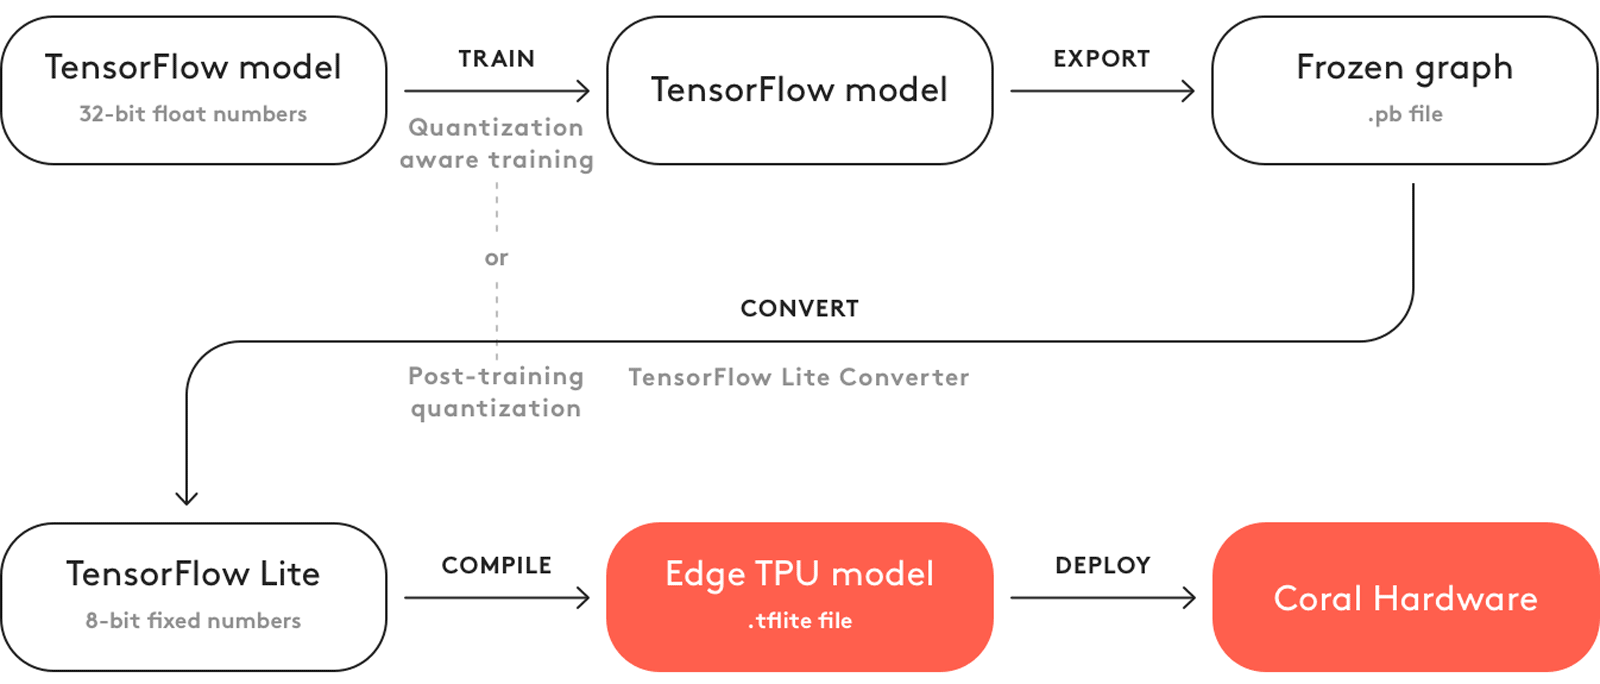
\includegraphics[width=\textwidth]{files/Edge_TPU_quantization.png}
  \caption{The basic workflow to create a model for the Edge TPU}
  \label{fig:quantization-chart}
\end{figure}

\section{Design}

\subsection*{Data}

To efficiently utilize \gls{tf}'s dataset loading and preprocessing capabilities, a versatile data handling method has to be implemented.
A core idea behind this approach is to unify the preparation of training, validation and test subsets within a single configurable function.
This function must manage all aspects of dataset construction and transformation according to user-defined parameters, thereby ensuring consistensy and flexibility.
The function should output \code{tf.data.Dataset} objects \cite{tfDataset} that are ready for immediate use in training pipelines. \cite{tfPaper}
\todo{cite main tf paper somwhere else earlier}

Ideally, the testing pipeline should also be incorporated within this flexible, unified function.
The absence of pre-cropped test subset \gls{gt} patches introduces the necessity for additional preparation steps.

\subsection*{Model}

%Separate from the dataset pipeline, the model architecture is developed independently.
The model architecture is tailored for deployment on embedded systems, where \gls{qat} must be taken into account.
Due to the lack of existing practical examples for deploying this specific model architecture on \gls{edgetpu},
the design process begins with a minimal configuration, using the smallest feasible number of layers and filters,
and gradually increases in complexity based on deployment outcomes and evaluation feedback.
An iterative, trial-and-error methodology is employed, allowing for adjustments in response to the resource constrains encountered on embedded hardware.

The objective is to implement multiple configurable functions, each responsible for constructing a distinct model architecture.
These functions include all necessary helper routines and utilities required to assemble the desired architecture,
allowing convenient switching between models during training.
%These limitations necessitate such architectural decisions, as the use of \gls{qat}.
%For this purpose, model layers are annotaded appropriately to support later quantization and efficient deployment on hardware with limited resources.

\subsection*{Training}
\label{subsec:designtrain}

After implementing utilities for dataset construction and defining the model architecture, the next step is to develop the training pipeline.
Initially, a simple and direct training pipeline should be created to validate basic model architectures, as a minimal setup both reduces potential error sources and enables rapid proof-of-concept.
During early development, model conversion is performed separately after training, before deployment.

However, the pipeline should be further refined, ideally as a single executable script, that encompasses data loading, training, configuration management, and model conversion,
streamlining the path to deployment. The goal is to enable a convenient, one-click training and conversion workflow.

To ensure reproducibility and facilitate backups, it is important to store all training configurations, logs, and intermediate model weights for each run.

Finally, computational resources must be considered. To avoid prohibitively long training times, the use of more powerful machines or cloud-based resources should be evaluated.

\subsection*{Conversion}

After training, the model must be converted and compiled for \gls{edgetpu} inference.
A modular approach is important here as well, simplifying debugging and ensuring correct conversion and compilation during early development.
Later, as described in \secshortref{subsec:designtrain}, integration of the conversion process directly into the training pipeline is ideal for convenience and efficiency.

Automation of the \gls{edgetpu} compiler,
provided by Google\footnote{\url{https://coral.ai/docs/edgetpu/compiler/}},
is required so that the entire training and conversion pipeline outputs a model ready for deployment on the \gls{devboard}.

\subsection*{Deployment}
\label{subsec:designdep}



\subsection*{Evaluation}
I wanna first conveniently have training, validation and test datasets ready for efficient TF training.
Then the convenient model architecture builder needs to be implemented
quantization aware training and post training quantization should be considered

}
{

\setlength{\parindent}{0pt}
\setlength{\parskip}{1em}

\chapter{Implementation}
\label{chapter:implementation}

A detailed description of the software development process used to achieve the thesis objective is provided in this chapter.
Along the way, three major implementation milestones were reached. Despite several hurdles, success was achieved in
(i) training the model on powerful cloud machines, (ii) mapping its all components, fully quantized, to the \gls{edgetpu},
and (iii) performing C++ inference on the \gls{devboard}.
The technical obstacles and their resolution are presented in three “Technical Challenges” chapters inside
\nameref{sec:training}, \nameref{sec:conversion}, and \nameref{sec:deployment}.

Software developed in the scope of this work
is made available for free and unrestricted use on the author's GitHub and TU Berlin GitLab profiles:
\begin{itemize}
  \item \url{https://github.com/An3Zh/BachelorThesis}
  \item GitLab link
\end{itemize}

Details on relevant file locations, with references to this work's chapters,
as well as further information on the repository structure, are provided in \code{README.md}.

\section{Data}
\label{sec:data}

\subsection{Training \& Validation}

In order to construct the training and validation pipeline, the function \code{BuildDS} was implemented, along with several supporting helper functions, all located in the \code{load.py} file.
The function was later extended to optionally include the test dataset, which will be discussed in \secshortref{subsec:testing}.

Efficient data handling and memory management are achieved through the use of built-in \gls{tf} utilities.
In particular, the \code{tf.Data.TextLineDataset}\footnote{\url{https://www.tensorflow.org/api_docs/python/tf/data/TextLineDataset}} function
is employed to sequentionally read the \code{.csv} files,
which contain the patch filenames as outlined in \secshortref{subsec:dataset}.
This provides the foundation for the dataset pipeline.

The complete training set originally contains 8400 patches. However, as explained earlier in \secshortref{subsec:dataset}, some patches are entirely zero-valued.
Only 5155 of them contain valid data and are thus retained for subsequent use.
The dataset is shuffled and split into training and validation subsets, with the ratio configurable as needed.

Using the \code{.map} method, each text line is first expanded into five full paths to the corresponding \gls{rgb}, \gls{nir} and \gls{gt} mask patches.
Each filepath is then replaced by its image content, loaded as \code{tf.Tensor}\footnote{\url{https://www.tensorflow.org/api_docs/python/tf/Tensor}}.
This transformation is handled by the helper function \code{loadDS}, which itself calls utility function \code{loadTIF}.
At this stage, each dataset element is a tuple of \gls{tf} tensors representing the four-channel input image and its corresponding \gls{gt} mask.

The \code{loadDS} and \code{loadTIF} functions perform the following operations:

\begin{itemize}
    \item RGB and NIR patches are cast to \gls{float32} and normalized to the range [0,1].
    \item \gls{gt} masks, originally in \gls{uint8}, are binarized to values of 0 and 1, and also cast to \gls{float32}.
\end{itemize}

An additional feature of the \code{loadDS} function allows for optional resizing of the input images if a target size is provided.
The image loading and transormation pipeline is designed to avoid information loss until the controlled resizing step, where a reduction in resolution is intentional.
In the case of resizing, \gls{gt} masks are resized using nearest-neighbor interpolation. This method copies the value of the closest original pixel for each target pixel,
thus preserving hard edges in the cloud segmentation mask and avoiding the introduction of intermediate values.
Conversely, the \gls{rgb} and \gls{nir} inputs are resized with bilinear interpolation,
which computes each new pixel value as a weighted average of the nearest $2\times2$ neighborhood. This results in smooth pixel transitions while maintaining important image details.
Nearest-neighbor interpolation is among the eraliest digital image resizing techniques, dating back to the origins of digital image processing in the 1960s,
whereas bilinear interpolation gained prominence in early computer graphics literature and is now standard in deep learning pipelines \cite{bilinearNearest1, bilinearNearest2}.

As a final preparation step, the dataset is: shuffled, batched, set to repeat indefinitely,
and prefetched to optimize data retrieval during training.
Because the datasets are repeated indefinitely, it is essential to define the number of steps required to complete one full pass through the training and validation subsets.
These step counts are used to ensure the correct number of iterations per epoch during training,
and they are computed as follows: \code{trainSteps(valSteps)~=~trainSubsetSize(valSubsetSize)~/~batchSize}.

\subsection{Testing}
\label{subsec:testing}

An additional capability of the \code{buildDS} is the construction of the test dataset.
As outlined in \secshortref{subsec:dataset}, only cropped \gls{rgb} and \gls{nir} test patches, together with complete scene \gls{gt} masks, are available for testing.
This arrangement necessitates two specific preparation steps prior to building the test pipeline:

\clearpage
\begin{enumerate}
    \item \textbf{Metadata collection:} To uniquely identify each scene, the \code{sceneID} is introduced, derived from the Landsat 8 metadata (path/row),
    and is unique within this test dataset. The total number of patches, as well as the number of rows and columns for each scene, is collected for every \code{sceneID}.
    The patch filenames, as outlined in \secshortref{subsec:dataset}, are used for this process.
    Additional \code{.csv} files were manually created --- each containing the ordered patch filenames corresponding to every full scene.
    Filenames in these \code{.csv} files are organized in the order resulting from cropping (left to right, top to bottom).
    Furthermore, the \code{fullTestDS.csv} file was generated, containing ordered patch filenames for all 20 full scenes.
    These \code{.csv} files, not provided in the original dataset,
    were developed in the scope of this thesis to support the test pipeline and are stored in the \code{additionalCSVs} folder within the testing subset.
    Based on this manually collected metadata, the \code{getSceneGridSizes} function was implemented in \code{load.py} file,
    returning a dictionary that maps each of the 20 \code{sceneID}s to the respective number of rows and columns in each scene.
    \item \textbf{Patch stitching:} The \code{stitchPatches} function was implemented in \code{load.py}.
    This function uses the \code{.csv} files and the \code{getSceneGridSizes} function to reconstruct entire scenes from the model's output patches for evaluation.
    The function can operate in two modes: it can either stitch together all scenes at once, saving all 20 full scenes,
    or stitch only a single specified scene. The single-scene mode is intended for debugging and verification, avoiding time-consuming processing of the full test subset.
\end{enumerate}

Following these preparatory steps, the \code{buildDS} function was extended with additional functionality to construct the test subset.
Using the optional boolean parameter \code{includeTestDS}, which indicates whether to include the test dataset, and the parameter \code{singleSceneID},
which allows the selection of a specific scene, the function now supports multiple modes for testing:

\begin{itemize}
    \item Utilizing all 9201 patches from the 20 test scenes, or
    \item Selecting patches from a single scene, either by specifying its \code{singleSceneID} or allowing the function to randomly select one.
    %based on pre-generated \code{.csv} files that map patch names to \code{sceneID}.
\end{itemize}

The dataset is then constructed using the same \gls{tf} utilities employed for the training and validation subsets.
It is important to emphasize that the test set is not shuffled, as preserving the initial patch order is essential for the subsequent stitching process.

Consequently, the \code{buildDS} function returns the training and validation subsets, along with their respective step counts based on the \code{batchSize}.
Optionally, it also returns test subset, which may contain either the entire test dataset or a single scene.
After inference, the model's output patches can be passed to the \code{stitchPatches} function, which reconstructs and saves the final scene images for further evaluation.

\clearpage
\section{Model}
\label{sec:model}

The core building blocks and utility functions for architecting the model are organized in \code{model.py}.
\gls{cnn} layers are constructed using \gls{tf}'s built-in \glspl{api}, allowing for a modular and reusable design.

In early development, the \code{simple} model architecture was implemented.
It served as a proof of concept and was used for initial debugging of the training and conversion pipelines, as well as to obtain the first inference results on the \gls{devboard}.
The model was not annotated for \gls{qat}.

Below in \autoref{fig:quantnotquantcomp} are schown the examples of layer diagrams for two models: the left is not annotated for \gls{qat}, the right is annotated.
These visualizations were produced with Netron\footnote{\url{https://netron.app/}}.
Following the concept outlined in \secshortref{subsubsec:qat}, the \code{QuantizeWrapperV2} and \code{QuantizeLayer} \glspl{tfop} are inserted into the architecture,
wrapping the base layers with quantize-dequantize operations.

\begin{figure}[H]
  \centering
  \begin{subfigure}[t]{0.48\textwidth}
    \centering
    \includegraphics[height=12cm]{files/modelPart.pdf}
    \caption{model part not annotated for \protect\gls{qat}}
  \end{subfigure}
  \hfill
  \begin{subfigure}[t]{0.48\textwidth}
    \centering
    \includegraphics[height=12cm]{files/modelPartQ.pdf}
    \caption{model part annotated for \protect\gls{qat}}
  \end{subfigure}
  \caption{Model before and after \protect\gls{qat} annotation}
  \label{fig:quantnotquantcomp}
\end{figure}

It is important to emphasize that \gls{bn} is applied to the output of the \code{Conv2D} \gls{tfop} and precedes the corresponding \code{Activation} function \cite{batchnormActivation}.

Subsequently, more complex \code{U-Net} architectures were implemented, with greater depth and skip connections.
Early versions of these models were not \gls{qat} annotated, instead, \gls{ptq} was applied at conversion time.

Where standard \gls{tf} loss functions are insufficient, custom losses such as \code{softJaccardLoss} and \code{diceLoss} are implemented in this module.
Custom metrics, particularly those used for segmentation evaluation and referenced in \autoref{subsec:evalmetrics}, are also provided within the \code{model.py} file.

\section{Training}
\label{sec:training}

The complete model training and conversion pipeline is implemented in the \code{main.py} file.

The process begins with configuration settings, which include:
\begin{itemize}
\item Batch size for training
\item Image size for both training and inference
\item Number of training epochs
\item Selected model architecture
\item Ratio between validation and training subsets
\item Number of batches used for the calibration dataset
\end{itemize}
Additional settings can be incorporated as needed.

The pipeline starts by loading the dataset using functions from \code{load.py}.
The selected model architecture is then compiled utilizing utilities from \code{model.py}.

Each training run is stored in a dedicated folder, named with a timestamp corresponding to the start of the run.
This folder contains all configuration files, training-related artifacts, and final results, including the compiled \gls{edgetpu} model.

Prior to training, the following configurations and callbacks are set up:

\begin{itemize}
\item \textbf{Model Checkpoints}: Model checkpoints are saved during training whenever the validation loss improves, preserving the best-performing model.
\item \textbf{Early Stopping}: If the validation loss stops improving, training continues for a predefined number of additional epochs before termination.
\item \textbf{Learning Rate Reduction}: The learning rate is reduced if the validation loss does not improve for a set number of epochs, helping to fine-tune convergence.
\end{itemize}

Once all configurations are saved, model training is initiated with the specified callbacks active.

Upon completion of training, the final model weights are saved and immediately used for model conversion.

\subsection*{Technical Challenges}

Training of initial proof-of-concept models was performed on a personal workstation equipped with an Intel Core i5-13400F \gls{cpu} and an NVIDIA GeForce RTX 4060 \gls{gpu}.
To enable \gls{gpu} acceleration for the \gls{tf} training process, the NVIDIA \gls{cuda} \gls{api} and the corresponding \gls{cudnn} library must be installed and configured.
The following versions were used: \gls{cuda} v11.2 and \gls{cudnn} v8.1.1.
These versions are not the latest available from NVIDIA at the time of this work, but were selected for compatibility with certain \glspl{tfop} and the \code{libedgetpu} runtime library.
Further details on these compatibility considerations are discussed in \secshortref{sec:conversion} and \secshortref{sec:deployment}.

Initial models containing approximately 300,000 parameters were trained without \gls{qat} for tens of epochs.
On the described setup and using the full training dataset, the time required for a single epoch was less than 15 seconds, which was deemed acceptable.

With the introduction of more complex models containing 2,000,000 and 30,000,000 (experimental, proven to be inefficient at edge inference) parameters,
and when employing \gls{qat}, training times increased significantly.
For these larger models, one epoch on the full training dataset required approximately 3 minutes and 12 minutes, respectively.
Since at least 100 epochs were necessary to achieve adequate model performance, more powerful hardware resources became essential.

Thunder Compute\footnote{\url{https://www.thundercompute.com/}}, an American startup with \gls{gpu} cloud resources for machine learning and data science,
provided solutions for large-scale experiments.
By using an instance with an NVIDIA A100XL \gls{gpu}, training times for the 2,000,000 parameter network were reduced to approximately 20 seconds per epoch,
and for the 30,000,000 parameter network to 40 seconds per epoch.
A \ensuremath{10\times} increase in \gls{gpu} memory, to 80GB on the A100XL compared to 8GB on the RTX 4060, also enabled larger batch sizes,
resulting in more effective training and improved model robustness.

However, significant effort was required to configure the cloud instance for compatibility.
The more expensive production mode\footnote{\url{https://www.thundercompute.com/docs/production-mode}} had to be used,
as the prototyping mode\footnote{\url{https://www.thundercompute.com/docs/prototyping-mode}} did not allow downgrading \gls{cuda} and \gls{cudnn} versions.
The \gls{cuda} and \gls{cudnn} libraries needed to be downgraded from their most recent platform versions to those compatible with an older \gls{tf} version.
This was challenging, as it required purging the latest \gls{cuda} and \gls{cudnn} files without removing the \gls{gpu} drivers required by the older versions.
Ultimately, \gls{cuda} v11.2 and \gls{cudnn} v8.1.0 were installed on the instance for subsequent training.
In addition, the Thunder Compute development team was contacted with a suggestion to allow selection of \gls{cuda} and \gls{cudnn} versions at instance creation.
As a result, an improvement is planned that will allow passing the desired \gls{cuda} and \gls{cudnn} version as an environment variable during instance startup.

\section{Conversion}
\label{sec:conversion}

The file \code{convert.py} contains all necessary functions and utilities for model conversion and \gls{edgetpu} compilation.
These functions are called from \code{main.py} immediately after training is complete.

\subsection{Weight Transfer}

As outlined in \secshortref{subsec:hardware}, the \gls{edgetpu} supports input tensors with at most three dimensions.
This necessitates the use of batch size one, since the input tensor shape is already \ensuremath{image~height~\times~image~width~\times~number~of~channels}.
During training, larger batch sizes are typically used for efficiency.
Therefore, after training, the function \code{asBatchOne} is used to transfer the trained weights to a model with identical architecture,
but with batch size set to one for the input, all intermediate computations, and the output.

\subsection{Post-Training Quantization}

The \code{tf.lite.TFLiteConverter}\footnote{\url{https://www.tensorflow.org/api_docs/python/tf/lite/TFLiteConverter}} utility is used to perform \gls{ptq} and convert the model into
the \code{.tflite} format.
A representative dataset, consisting of training \gls{rgb} and \gls{nir} patches, is generated using the \code{representativeDatasetGen} function.
The number of calibration batches used can be adjusted via \code{numCalBatches}, as defined in \secshortref{sec:training}.
The greater the amount of calibration data, the more likely the observed value range will closely match the inference data, improving quantization accuracy.

As a next step, all supported \glspl{tfop} as well as model inputs and outputs are quantized.
While various data types can be used for quantization in general case,
this work utilizes \gls{int8}, as required for \gls{edgetpu} compatibility in \secshortref{subsec:hardware}.

The following subchapter provides a deeper investigation into quantization of model parameters by analyzing a \gls{qat}-annotated \gls{float32} model and its already quantized version.
The Netron tool is used here as well for visualizing the model's parts.
This chapter is aimed at readers who wish to deepen their understanding of parameter quantization and gain insight into the general techniques
behind full-integer operation execution on edge devices such as the \gls{edgetpu}.

It should be noted that both \gls{qat} annotation and \gls{ptq} are already wrapped into convenient, ready-to-use \gls{tflite} commands.
Thus, this section is not intended to teach the implementation of quantized models from scratch. Instead, it aims to offer a deeper understanding that can be beneficial for debugging, designing custom (potentially more powerful) models, or simply appreciating the engineering trade-offs between speed, memory, and accuracy on constrained devices.

\subsection{Practical example of Model quantization}
\label{subsubsec:optquant}

Below, a \gls{qat} annotated part of the model is shown in the left panel of \autoref{fig:qatconvertedquant}.
On the right, the same part is shown after \gls{ptq}, yielding a fully \gls{int8} quantized model.

\begin{figure}[H]
  \centering
  \begin{subfigure}[t]{0.48\textwidth}
    \centering
    \includegraphics[height=12cm]{files/modelPartQBeforePTQ.pdf}
    \caption{model part annotated for \protect\gls{qat}}
  \end{subfigure}
  \hfill
  \begin{subfigure}[t]{0.48\textwidth}
    \centering
    \includegraphics[height=12cm]{files/modelPartQAfterPTQ.pdf}
    \caption{model part after full \protect\gls{int8} quantization}
  \end{subfigure}
  \caption{Model before and after quantization}
  \label{fig:qatconvertedquant}
\end{figure}

Netron also provides detailed information about graph nodes (model layers) and their connections (tensor passes).
For example, layer weights and biases can be directly inspected, and values can be examined.
In the tables below, quantization-relevant information is displayed for further analysis.

For both the \gls{qat} annotated model and the resulting quantized model, the relevant information for four layers is summarized.
All floating-point numbers are shown in full \gls{float32} precision.
Representative calculations are performed in full precision and displayed with extended decimals.
The goal is to illustrate, using a practical example, the error effects of quantization and the limits of \gls{float32} precision.

\clearpage
\subsubsection*{\gls{qat} Annotated Model (left in \autoref{fig:qatconvertedquant})}

\begin{layerbox}{Layer Type: QuantizeLayer}{Layer Name: Quantize Input}
  \begin{center}
    \textbf{Input value range:} \\[2pt]
    $\min = 0 \quad\quad \max = 1$
  \end{center}
\end{layerbox}

\begin{layerbox}{Layer Type: QuantizeWrapperV2}{Layer Name: Conv2D No. 1}
  \begin{center}
    \textbf{Kernel shape:} \\[2pt]
    $[3, 3, 4, 32]$ \\[6pt]
    \textbf{Kernel No. 1 value range:} \\[2pt]
    $\min = -0.544256329536438 \quad\quad \max = 0.544256329536438$ \\[6pt]
    \textbf{First element of Kernel No. 1 value:} \\[2pt]
    $0.032761260867118835$ \\[6pt]
    \textbf{Bias shape:} \\[2pt]
    $[32]$ \\[6pt]
    \textbf{Bias No. 1 value:} \\[2pt]
    $0.1983194351196289$ \\[6pt]
    \textbf{Activation value range:} \\[2pt]
    $\min = -2.4379329681396484 \quad\quad \max = 1.0039010047912598$
  \end{center}
\end{layerbox}

\begin{layerbox}{Layer Type: \glsxtrlong{bn}}{Layer Name: \gls{bn} No. 1}
  \begin{center}
    \textbf{Shape of $\gamma$, $\beta$, $\mu_{\text{moving}}$, $\sigma^2_{\text{moving}}$ parameters:} \\[2pt]
    $[32]$ \\[6pt]
    \textbf{Parameter $\gamma_1$ value:} \\[2pt]
    1.110548973083496 \\[6pt]
    \textbf{Parameter $\beta_1$ value:} \\[2pt]
    -0.11593257635831833 \\[6pt]
    \textbf{Parameter $\mu_{\text{moving},1}$ value:} \\[2pt]
    0.17263321578502655 \\[6pt]
    \textbf{Parameter $\sigma^2_{\text{moving},1}$ value:} \\[2pt]
    0.00221889466047287
  \end{center}
\end{layerbox}


\begin{layerbox}{Layer Type: QuantizeWrapperV2}{Layer Name: Activation No. 1}
  \begin{center}
    \textbf{Output value range:} \\[2pt]
    $\min = -3.696099329375535 \mathrm{e}{-11} \quad\quad \max = 18.816810607910156$
  \end{center}
\end{layerbox}

\clearpage
\subsubsection*{Model After Quantization (right in \autoref{fig:qatconvertedquant})}

\begin{layerbox}{Layer Type: Conv2D}{Layer Name: Conv2D No. 1}
  \begin{center}
    \textbf{Input affine dequantization formula:} \\[2pt]
    $x_{\text{q}} \approx 0.003921568859368563 \times (q_{\text{x}} + 128)$ \\[6pt]
    \textbf{Kernel No. 1 symmetric dequantization formula:} \\[2pt]
    $x_{\text{q}} \approx 0.004285482689738274 \times q_{\text{x}}$ \\[6pt]
    \textbf{First element of Kernel No. 1 quantized value:} \\[2pt]
    $8$ \\[6pt]
    \textbf{Bias No. 1 symmetric dequantization formula:} \\[2pt]
    $x_{\text{q}} \approx 0.000016805815903353505 \times q_{\text{x}}$ \\[6pt]
    \textbf{Bias No. 1 quantized value:} \\[2pt]
    $11801$ \\[6pt]
  \end{center}
\end{layerbox}

\begin{layerbox}{Layer Type: Mul}{Layer Name: \gls{bn} No. 1 Scale}
  \begin{center}
    \textbf{Input affine dequantization formula:} \\[2pt]
    $x_{\text{q}} \approx 0.013497387990355492 \times (q_{\text{x}} - 53)$ \\[6pt]
    \textbf{Fused \gls{bn} multiplier $M_c$ affine dequantization formula:} \\[2pt]
    $x_{\text{q}} \approx 0.10698594152927399 \times (q_{\text{x}} + 128)$ \\[6pt]
    \textbf{Multiplier $M_1$ quantized value:} \\[2pt]
    $55$ \\[6pt]
  \end{center}
\end{layerbox}

\begin{layerbox}{Layer Type: Add}{Layer Name: \gls{bn} No. 1 Shift}
  \begin{center}
    \textbf{Input affine dequantization formula:} \\[2pt]
    $x_{\text{q}} \approx 0.17354172468185425 \times (q_{\text{x}} - 26)$ \\[6pt]
    \textbf{Fused \gls{bn} additive term $A_c$ affine dequantization formula:} \\[2pt]
    $x_{\text{q}} \approx 0.0339626707136631 \times (q_{\text{x}} + 10)$ \\[6pt]
    \textbf{Additive term $A_1$ quantized value:} \\[2pt]
    $-113$ \\[6pt]
  \end{center}
\end{layerbox}

\begin{layerbox}{Layer Type: ReLU}{Layer Name: Activation No. 1}
  \begin{center}
    \textbf{Output affine dequantization formula:} \\[2pt]
    $x_{\text{q}} \approx 0.07379141449928284 \times (q_{\text{x}} + 128)$ \\[6pt]
  \end{center}
\end{layerbox}

\clearpage
Before presenting the calculations, the Quantization Specification Table\footnote{\url{https://ai.google.dev/edge/litert/models/quantization_spec}} is reviewed.
An excerpt relevant to the \gls{tfop} \code{Conv2D} is shown below:

\begin{verbatim}
CONV_2D
  Input 0:
    data_type  : int8
    range      : [-128, 127]
    granularity: per-tensor
  Input 1 (Weight):
    data_type  : int8
    range      : [-127, 127]
    granularity: per-axis (dim = 0)
    restriction: zero_point = 0
  Input 2 (Bias):
    data_type  : int32
    range      : [int32_min, int32_max]
    granularity: per-axis
    restriction: (scale, zero_point) = (input0_scale*input1_scale[...], 0)
  Output 0:
    data_type  : int8
    range      : [-128, 127]
    granularity: per-tensor
\end{verbatim}

Using this information, quantization calculations can be retraced for a better understanding of model transformation.
The \code{input\_1} values, or the model's input tensors, are observed first from the \code{QuantizeLayer}.
As expected, these range from 0 to 1 due to normalized input patches.

The input scale and zero-point can be calculated using equations \ref{eq:scale} and \ref{eq:zeropoint} from \secshortref{subsec:quantization}:

\[
\begin{array}{rl}
\text{Input scale} &= \dfrac{1 - 0}{127 - (-128)} = 0.003921568627450980 \\[16pt]
\text{Input zero-point} &= \text{round}\!\left(-128 - \dfrac{0}{\text{Input scale}}\right) = -128
\end{array}
\]

The calculated values align with the "Input affine dequantization formula" for the \code{Conv2D} layer in the quantized model.
The precision difference at the 10th decimal place is expected due to \gls{float32} limits.
This confirms the use of affine (asymmetric) quantization for \code{Input 0},
consistent with the table's range [-128,127] and the absence of a zero-point restriction.

Moving to the \code{Conv2D} layer weights, the table specifies per-axis granularity with symmetric quantization (zero-point=0).
Inspection of the 32 kernel value ranges (only Kernel No. 1 shown here) confirms symmetry around zero.
This suggests that \gls{tf} enforces clipping of weight extremes to fit symmetric ranges.

Netron reveals that Kernel No. 1 has the largest max value among the 32 kernels (not represented here),
yet it still doesn't match the actual tensor extrema ($min=-0.4122757017612457, max=0.5442604422569275$),
indicating that \gls{tf} may apply additional optimization, likely outlier-aware clipping or mean adjustment,
since real values are not perfectly zero-mean ($mean=-0.005126346834471305$).
A detailed investigation of this effect lies outside the scope of this work.

Using the clipped extrema, the symmetric quantization scale is:

\[
\begin{array}{rl}
\text{Kernel No. 1 scale} &= \dfrac{0.544256329536438 - (-0.544256329536438)}{127 - (-127)}\\[8pt]
                          &= 0.004285482909735732
\end{array}
\]

This matches the Kernel No. 1 symmetric dequantization formula from the quantized model (within \gls{float32} precision limits).
Applying equation \ref{eq:dequantize}, the quantized value can be approximately dequantized back to the first element of Kernel No. 1:

\[
\begin{array}{rl}
\text{First element of Kernel No. 1} \approx 0.004285482689738274 \cdot 8 = 0.034283861517906192
\end{array}
\]

The resulting precision loss is small and can be quantified by absolute, relative, and \gls{lsb} errors:

\begin{itemize}[itemsep=0.4\baselineskip]
    \item $e_{\text{abs}} = 0.034283861517906192 - 0.032761260867118835 = 0.001522600650787357$
    \item $e_{\text{rel}} = \frac{0.001522600650787357}{0.032761260867118835} \times 100\% \approx 4.647\%$
    \item $e_{\text{lsb}} = \frac{0.001522600650787357}{0.004285482689738274} \approx 0.355,\ \Delta = 0.004285482689738274$
\end{itemize}

Here, the \gls{lsb} error $<0.5$ is a good indicator: it suggests that scale boundaries are not exceeded and quantization was applied without mismatches,
clipping errors, or encoding/decoding inconsistencies.

Looking at the bias restrictions in the Quantization Specification Table, an interesting point emerges:
the bias has no dedicated quantization scale derived from its own extrema.
Hence, no min/max values are logged by \code{QuantizeWrapperV2} for the \code{Conv2D} layer.
Instead, its scale is computed as the product of the layer's input scale and the per-channel weight scale,
yielding one bias scale per output channel (matching the weight scales per axis).
This engineering choice accelerates inference at the cost of a slight precision loss.

Multiplying input values by weights (each with its own scale) produces a new effective scale.
To add the bias to this product, the bias must be quantized using the same scale (with zero-point=0).
One could quantize the bias with its own scale and then rescale the product accordingly,
but this introduces extra operations that would significantly slow inference.
Instead, fast fixed-point arithmetic is employed, using a precomputed quantized multiplier and a bit-shift,
to reconcile the mixed scales that arise when multiplying quantized values.

\[
\begin{array}{rl}
\text{Bias No. 1 scale} &= 0.003921568859368563 \cdot 0.004285482689738274 \\
             &= 0.0000168058154634406445 \\[8pt]
\text{Bias No. 1 value} &\approx 0.000016805815903353505 \cdot 11801 \\
      &= 0.198325433475474713
\end{array}
\]

Analogous calculations can be performed for the Bias No. 1 to determine its scale and recover its approximate \gls{float32} value.

As can be seen in the Netron analysis, the \gls{bn} \gls{tfop} is decomposed into two primitive \glspl{tfop} after quantization: \code{Mul} and \code{Add}.
This follows from the affine form of batch normalization (and its folding during quantization), which can be expressed as:

\begin{equation}
y = \gamma \cdot \frac{x - \mu_{\text{moving}}}{\sqrt{\sigma^2_{\text{moving}} + \epsilon}} + \beta
\label{eq:bn}
\end{equation}

\begin{equation}
M_c = \frac{\gamma_c}{\sqrt{\sigma^2_{\text{moving},c} + \epsilon}}, 
\quad
A_c = \beta_c - \frac{\gamma_c \cdot \mu_{\text{moving},c}}{\sqrt{\sigma^2_{\text{moving},c} + \epsilon}}
      = \beta_c - M_c \cdot \mu_{\text{moving},c}
\label{eq:bnquant}
\end{equation}

\begin{itemize}
    \item \textbf{$x$}: input value to be normalized.
    \item \textbf{$y$}: output value after batch normalization.
    \item \textbf{$\mu_{\text{moving},c}$}: moving mean for channel $c$, computed during training as an exponential moving average of per-batch means; used in inference because batch statistics from a single sample are often unreliable.
    \item \textbf{$\sigma^2_{\text{moving},c}$}: moving variance for channel $c$, computed during training as an exponential moving average of per-batch variances; also used in inference for the same reason as the moving mean.
    \item \textbf{$\epsilon$}: small constant to avoid division by zero (default\footnote{\url{https://www.tensorflow.org/api_docs/python/tf/keras/layers/BatchNormalization}} \gls{tf} value is set to 0.001).
    \item \textbf{$\gamma_c$}: learnable scale parameter for channel $c$.
    \item \textbf{$\beta_c$}: learnable shift parameter for channel $c$.
    \item \textbf{$M_c$}: per-channel multiplier used in quantized inference.
    \item \textbf{$A_c$}: per-channel additive term used in quantized inference.
\end{itemize}

It should be noted that the affine dequantization of the \code{Mul} input is computed from the extrema of the outputs of \code{Conv2D} No.~1,
analogous to the previous calculations of scales and zero-points.

In quantized form, $\mu_{\text{moving}}$, $\sigma^2_{\text{moving}}$, $\gamma$, and $\beta$ are fused into per-channel multiplier $M_c$ and additive term $A_c$.
Reverse-engineering from the quantized values recovers the original \gls{float32} parameters with minimal error:

\begin{equation*}
\begin{gathered}
M_1 = 0.10698594152927399 \cdot (55 + 128) \approx 19.5784273 \\
\sqrt{\sigma^2_{\text{moving},1} + \epsilon} = \sqrt{0.00221889466047287 + 0.001} \approx 0.0567353 \\
\hat{\gamma}_1 = M_1 \cdot \sqrt{\sigma^2_{\text{moving},1} + \epsilon} \approx 19.5784273 \times 0.0567353 \approx 1.1107880 \\
\hat{\gamma}_1 = 1.1107880 \approx \gamma_1 = 1.110548973083496
\end{gathered}
\end{equation*}


\begin{equation*}
\begin{gathered}
A_1 = 0.0339626707136631 \cdot (-113 + 10) \approx -3.4981550 \\
\beta_1 = A_1 + M_1 \cdot \mu_{\text{moving},1} \approx -3.4981550 + 19.5784273 \times 0.1726332 \approx -0.1182682 \\
\beta_1 = -0.1182682 \approx \beta_{1,\text{float}} = -0.11593257635831833
\end{gathered}
\end{equation*}

Finally, the "Output affine dequantization formula" is derived from the extrema of the (ReLU) Activation No. 1 layer:

\[
\begin{array}{rl}
\text{Output scale} &= \frac{18.816810607910156 - (-3.696099329375535 \mathrm{e}{-11})}{127 - (-128)} \\
             &= 0.073791414148812224 \\[8pt]
\text{Output zero-point} &= \text{round}\left( -128 - \frac{-3.696099329375535 \mathrm{e}{-11}}{\text{Output scale}} \right) \\
                  &= -128
\end{array}
\]


All subsequent quantization steps for \glspl{tfop} in the model follow the same general procedure, adhering to predefined constraints and reusing common underlying methods.

From this deeper investigation, the following key quantization principles emerge:
\begin{itemize}
    \item After \gls{ptq}, the \code{QuantizeInput} layer defines the input scale and input zero-point based on observed extrema.
    Same calculation principles apply further.
    \item Weights are typically quantized per-axis (per-channel) with symmetric ranges.
    \item Bias scales are derived from input and weight scales, enabling fixed-point computation without extra rescaling.
    \item Certain operations, such as \gls{bn}, are decomposed into simpler arithmetic operations for inference efficiency.
    \item The precision loss is small, and \gls{lsb} error below $0.5$ indicates well-matched scales.
\end{itemize}

After quantized model is saved, the \gls{edgetpu} Compiler is invoked.

\clearpage
\subsection{Edge TPU Compiling}

Since training may be performed either on a local Windows machine or on a Linux-based cloud \gls{gpu} instance from Thunder Compute,
cross-platform automation of the pipeline is ensured by using helper functions and platform detection before invoking the \gls{edgetpu} compiler.
Because the \gls{edgetpu} compiler can only run on Debian-based Linux systems, the Windows Subsystem for Linux (WSL) is used when working on a Windows machine.

The \gls{edgetpu} Compiler parses the \code{.tflite} model, verifies that the restrictions are satisfied and that it is compatible with the \gls{edgetpu} runtime,
and then attempts to fuse all supported \glspl{tfop} into a single \code{edgetpu-custom-op}.
An example of the compiler's console output during compilation is shown below.

\lstdefinestyle{compilerlog}{
  basicstyle=\normalsize\ttfamily, % can adjust \fontsize{12pt}{13.5pt}
  captionpos=b,                    % caption at the bottom
  frame=single,                     % box around the log
  breaklines=true,
  showstringspaces=false,
  columns=fullflexible
}

\begin{lstlisting}[style=compilerlog,
    caption={Edge TPU compiler console output. Successful compilation},
    label={lst:edgetpu_compilation}]
Edge TPU Compiler version 16.0.384591198
Started a compilation timeout timer of 180 seconds.

Model compiled successfully in 898 ms.

Input model: dev/results/run_20250719_170647/quant.tflite
Input size: 1.90MiB
Output model: dev/results/run_20250719_170647/quant_edgetpu.tflite
Output size: 2.07MiB
On-chip memory used for caching model parameters: 1.90MiB
On-chip memory remaining for caching model parameters: 3.82MiB
Off-chip memory used for streaming uncached model parameters: 46.00KiB
Number of Edge TPU subgraphs: 1
Total number of operations: 53
Operation log: dev/results/run_20250719_170647/quant_edgetpu.log
See the operation log file for individual operation details.
Compilation child process completed within timeout period.
Compilation succeeded!
\end{lstlisting}

The \gls{edgetpu} has \(\sim 8\,\mathrm{MiB}\) of static \gls{ram}, allowing model parameters to be cached.
It is further specified\footnote{\url{https://coral.ai/docs/edgetpu/compiler/\#parameter-data-caching}} that multiple models can be co-compiled and
stored in the \gls{edgetpu}'s on-chip memory, enabling fast switching and inference when different models are required on a single \gls{edgetpu}.
Conversely, a model can be partitioned for pipelining across multiple \glspl{edgetpu}, allowing parallel inference or acceleration of larger models.
In the scope of this thesis, however, only a single \gls{edgetpu} is used.
Therefore, the on-chip static \gls{ram} should ideally not be exceeded to preserve inference speed.
Falling back to external memory can degrade performance due to parameter reloads.

From the \autoref{lst:edgetpu_compilation} log example, useful information about memory usage can be inferred.
The model executable occupies approximately \(8 - 1.90 - 3.82 \approx 2.28\,\mathrm{MiB}\) of the \gls{edgetpu} on-chip cache.
Its parameters occupy \(1.90\,\mathrm{MiB}\), leaving \(3.82\,\mathrm{MiB}\) free, thus, the entire model is stored in the \gls{edgetpu}'s static \gls{ram}.
In \secshortref{chapter:evaluation}, memory usage is also considered when comparing different models.
For this particular model, however, \(46.00\,\mathrm{KiB}\) of external memory was still utilized despite the remaining free on-chip memory.
The reason is not documented officially and likely requires deeper investigation of the compilation process, which lies outside the scope of this thesis.

After successful compilation, a \code{.log} file is saved alongside the \gls{edgetpu} model.
This log reports, for each \gls{tfop}, whether mapping to the \gls{edgetpu} succeeded (and, if not, why),
as illustrated by the \code{.log} excerpt shown right in \autoref{fig:successcompile}.

One way to confirm that the entire model compiles for the \gls{edgetpu} is to visualize the compiled model in Netron.
An example demonstrating that every \gls{tfop} was successfully mapped to the \gls{edgetpu} is shown left in \autoref{fig:successcompile}.
In contrast to the pre-compilation graphs (for example, see \autoref{fig:qatconvertedquant}), no additional structural information is visible:
all supported \glspl{tfop} have been fused into a single \code{edgetpu-custom-op} that executes exclusively on the \gls{edgetpu}.
As shown, the input and output tensor shapes are readable, and the associated quantization scales and zero points can be inspected,
as in \secshortref{subsubsec:optquant}; no further details are exposed.

\begin{figure}[htbp]
\begin{minipage}[t]{0.26\textwidth}\vspace{0pt} % check line 552
    \centering
    % Scale the image to fit half page width while keeping aspect ratio
    \includegraphics[width=\linewidth,keepaspectratio]{files/EdgeTPUCompiledModel.pdf}
\end{minipage}%
\hspace{0.5cm plus 1fill} % if I use \hfill the overfull disappears 
\begin{minipage}[t]{0.74\textwidth}\vspace{0pt}
    \vspace*{\fill}        % push down from top
    \raggedright           % left-align text inside this block
    \small

    Edge TPU Compiler version 16.0.384591198\\
    Input: dev/results/run\_20250719\_170647/quant.tflite\\
    Output: dev/results/run\_20250719\_170647/quant\_edgetpu.tflite\\

    \vspace{0.5em}
    \begin{tabular}{@{}lrl@{}}
      Operator & Count & Status \\[0.5em]  % extra space after header row
      CONCATENATION & 3  & Mapped to Edge TPU \\
      LOGISTIC      & 1  & Mapped to Edge TPU \\
      ADD           & 14 & Mapped to Edge TPU \\
      MAX\_POOL\_2D & 3  & Mapped to Edge TPU \\
      MUL           & 14 & Mapped to Edge TPU \\
      CONV\_2D      & 15 & Mapped to Edge TPU \\
      TRANSPOSE\_CONV & 3 & Mapped to Edge TPU
    \end{tabular}
    \vspace*{\fill}        % push up from bottom -> vertical centering
\end{minipage}
\caption{\gls{edgetpu}-mapped model (left) and compiler log excerpt (right).}
\label{fig:successcompile}
\end{figure}

The final artifact is a \code{.tflite} model file ready for \gls{edgetpu} inference.

\subsection*{Technical Challenges}

The \gls{devboard} is running on an end of life version of Mendel Linux, which is the only one latest officialy supported software version for \gls{devboard}.
With the OS itself comes already pre-installed runtime library \code{libedgetpu} of version v16.0, exposing a low-level C++ \gls{api}
for direct interaction with \gls{edgetpu}. Consequently, this library version is the latest officially available in Coral repository for this Mendel Linux release.
Building the latest version from source entails a more complex Bazel-based process that risks breaking dependencies and incurs a nontrivial debugging burden; 
this lies outside the scope of this thesis.

The newest as of today \gls{edgetpu} Compiler version v16.0 is used,
requiring minimum\footnote{\url{https://coral.ai/docs/edgetpu/compiler/\#compiler-and-runtime-versions}} runtime version v14.0,
which is fulfilled by \code{libedgetpu} v16.0.

At early development stages, it was unclear which \gls{tf} version was supported by the provided runtime library and compiler,
as this information was not available in the official documentation.
Consequently, the newest \gls{tf} version, v2.19.0 (at the time this work was conducted), was used heuristically for initial attempts at dataset pipeline construction,
model architecture, training, and conversion.
No \gls{qat} annotation was performed, relying solely on \gls{ptq} prior to compiling the model for trial inference on the \gls{edgetpu}.
At compile time, the following error from the \gls{edgetpu} Compiler was encountered:

\begin{lstlisting}
Edge TPU Compiler version 16.0.384591198
ERROR: Didn't find op for builtin opcode 'TRANSPOSE_CONV' version '4'.
An older version of this builtin might be supported.
Are you using an old TFLite binary with a newer model?
\end{lstlisting}

To avoid this error, the first approach was to omit the \code{TRANSPOSE\_CONV} \gls{tfop} while keeping the newest \gls{tf},
replacing deconvolution with the simpler combination \code{UpSampling2D} + \code{Conv2D}.
This may reduce accuracy but could still yield acceptable results for edge-device inference. Alternatively,
the \gls{tf} version was downgraded to v2.5.0, corresponding to the \gls{tflite} library on the \gls{devboard},
to maximize version compatibility with the target hardware. After the downgrade, the first successful compilation and inference were achieved.
Results are presented in \secshortref{sec:evaluation}.

With the introduction of \gls{qat} annotated model layers, the \gls{tfmot} package must be installed, with a version compatible with \gls{tf} v2.5.0.
This required installing \gls{tfmot} v0.6.0.
During the \gls{tflite} conversion step (while performing \gls{ptq}), the following error kept occurring:

\begin{lstlisting}
error: 'tfl.max_pool_2d' op quantization parameters violate the same
scale constraint: !quant.uniform<i8:f32, 840332.86281612806:-128>
vs. !quant.uniform<i8:f32, 0.027852464160498452:-127>
\end{lstlisting}

This error refers to the \gls{tflite} restriction (see \secshortref{subsubsec:optquant}) that the inputs and outputs of \code{MAX\_POOL\_2D} must share the same scale and \code{zero\_point},
as specified in the Quantization Specification Table\footnote{\url{https://ai.google.dev/edge/litert/models/quantization_spec}}.
As part of debugging, it was verified that the input and output minimum and maximum ranges were essentially identical. Only the mean distributions differed,
which is normal for batches with different compositions:

\noindent
\begin{minipage}[t]{0.48\textwidth}
\begin{lstlisting}[basicstyle=\ttfamily\small\centering, columns=fullflexible, keepspaces=true, frame=single]
      ---- INPUT TO MAXPOOL ----
      Shape: (1, 384, 384, 16)
      min:   0.0
      max:   3.411252021789551
      mean:  1.003772497177124
\end{lstlisting}
\end{minipage}%
\hfill
\begin{minipage}[t]{0.48\textwidth}
\begin{lstlisting}[basicstyle=\ttfamily\small\centering, columns=fullflexible, keepspaces=true, frame=single]
      ---- OUTPUT OF MAXPOOL ----
      Shape: (1, 192, 192, 16)
      min:   0.0
      max:   3.411252021789551
      mean:  1.0165772438049316
\end{lstlisting}
\end{minipage}

Furthermore, a sanity check of the value ranges across different input batches was performed, confirming expected values from \(0\) to \(\sim 5\),
without extreme outliers, thus, there is no justification for very large scale \(840{\,}332.8\) as indicated by the error message.
Activation ranges of the preceding \code{Conv2D} layer were inspected in Netron and showed no anomalies.
These findings suggest an internal issue with this specific \gls{tfmot} version, as the observed input/output statistics contradict the scale values implied by the error message.

During debugging, it was further identified that a similar issue\footnote{\url{https://github.com/tensorflow/model-optimization/issues/1053}} had been reported for a later \gls{tfmot} version.
Combined with the observations above, this suggested trying a newer \gls{tfmot} release in which the bug might be fixed.
This raised concerns about compatibility with the older \gls{tf} v2.5.0 required for \gls{tflite} (\gls{tfop} v3) compatibility mentioned earlier.
It was decided to proceed, however, given the absence of documentation explicitly stating incompatibility of newer \gls{tfmot} with older \gls{tf}.
Multiple version combinations of these modules were evaluated.

Selecting a combination of newer \gls{tfmot} and \gls{tf} resolved the issue.
This, in turn, supports the conclusion that the error originated in the \gls{tf}/\gls{tfmot} implementation and was corrected in later releases.

Successful conversion to the \code{.tflite} format was subsequently achieved.
During conversion, the newer \gls{tf}/\gls{tfmot} toolchain automatically inserted a \code{Transpose} \gls{tfop} into the model.
This operator was not used during model design, indicating an internal optimization related to \gls{qat} handling.
A plausible explanation is the need to convert between common tensor layouts --- \code{[batch, H, W, C] (NHWC)} and \code{[batch, C, H, W] (NCHW)} --- at some point in the pipeline.
Limitations in one component's ability to process a given layout can trigger such a transformation, implemented as a \code{Transpose} placed before \code{TransposeConv}.
Below in \autoref{fig:transposeerror}, the same model architecture is shown before (left) and after (right) the \gls{edgetpu} compilation process.

\begin{figure}[H]
  \centering
  \begin{subfigure}[t]{0.48\textwidth}
    \centering
    \includegraphics[height=11cm]{files/modelPartQuantEdgeTPUFail.pdf}
    \caption{Before compilation}
  \end{subfigure}
  \hfill
  \begin{subfigure}[t]{0.48\textwidth}
    \centering
    \includegraphics[height=11cm]{files/modelPartCustomEdgeTPUFail.pdf}
    \caption{After compilation}
  \end{subfigure}
  \caption{Inserted \code{Transpose} \gls{tfop} prevents fusion into a single \code{edgetpu-custom-op}.}
  \label{fig:transposeerror}
\end{figure}

Both the crucial console output and the \code{.log} file are provided in \autoref{lst:edgetpu_compilation1},
indicating the failed attempt to fuse multiple \glspl{tfop} into the intended \code{edgetpu-custom-op}.

\begin{lstlisting}[
  basicstyle=\ttfamily\small,
  columns=fullflexible,
  keepspaces=true,
  showstringspaces=false,
  breaklines=false,      % don't wrap—preserves column layout
  frame=single,
  xleftmargin=0pt,
  linewidth=\textwidth,  % fill the page width
  caption={Failed mapping to \gls{edgetpu}},
  label={lst:edgetpu_compilation1},
  captionpos=b
]
Model successfully compiled but not all operations are supported
by the Edge TPU. A percentage of the model will instead run on the CPU,
which is slower. If possible, consider updating your model to use only
operations supported by the Edge TPU.
For details, visit g.co/coral/model-reqs.
Number of operations that will run on Edge TPU: 4
Number of operations that will run on CPU: 7
See the operation log file for individual operation details.

Logfile:
Edge TPU Compiler version 16.0.384591198
Input: quant.tflite
Output: quant_edgetpu.tflite

Operator             Count         Status
      
CONV_2D              2             More than one subgraph is not supported
CONV_2D              2             Mapped to Edge TPU
TRANSPOSE_CONV       1             Filter, bias, or other param is not
                                   constant at compile-time
LOGISTIC             1             More than one subgraph is not supported
ADD                  1             More than one subgraph is not supported
MAX_POOL_2D          1             Mapped to Edge TPU
CONCATENATION        1             More than one subgraph is not supported
TRANSPOSE            1             Tensor has unsupported rank
                                   (up to 3 innermost dimensions mapped)
QUANTIZE             1             Mapped to Edge TPU
\end{lstlisting}

This behaviour confirms that multiple layers of the model do not meet the requirements defined in \secshortref{subsec:hardware},
and it is consistent with the compilation procedure described in the official documentation\footnote{\url{https://coral.ai/docs/edgetpu/models-intro/\#compiling}}.
Specifically, the compiler stops at the first operation not supported by the \gls{edgetpu} and maps all subsequent operations to the \gls{cpu},
even if some of those later operations would otherwise be supported on the \gls{edgetpu}.
This behaviour is illustrated below in \autoref{fig:compileSeqEdgeTPU}.

\begin{figure}[htbp]
  \centering
  % Choose either a width OR a height, or both with keepaspectratio.
  % Example A: set width only (aspect ratio preserved automatically)
  \includegraphics[width=0.8\linewidth]{files/compileSequenceEdgeTPU.png}

  % Example B (recommended): limit both max width & height, keep aspect ratio
  %\includegraphics[
  %  width=0.9\linewidth,
  %  height=0.5\textheight,
  %  keepaspectratio
  %]{images/example.png}

  \caption{The compiler creates a single custom op for all \gls{edgetpu} compatible ops, until it encounters an unsupported op; the rest stays the same and runs on the \gls{cpu}}
  \label{fig:compileSeqEdgeTPU}
\end{figure}

Delegation of tensor operations to the \gls{cpu} will almost certainly increase inference time drastically, which is inappropriate here,
as the goal is to map the entire model to the \gls{edgetpu}.

Because insertion of the \code{Transpose} \gls{tfop} occurs entirely internally and automatically,
there is no practical way to influence it or to enforce layer parameters to be constant at compile time and of shape \(<3\), as required by the \gls{edgetpu} Compiler.

Two options were considered: (i) avoid \code{TransposeConv} altogether, or (ii) continue searching for compatible \gls{tf} and \gls{tfmot} versions.
Pursuing the second option places one between a rock and a hard place:
the \gls{tf} version should be kept as low as possible to maintain compatibility with the device \gls{tflite} runtime and
to avoid the previously observed \code{TRANSPOSE\_CONV} version 4 compiler error, yet sufficiently high to include the bug fix for the scale incompatibility encountered earlier.
Accordingly, the following approach was adopted: identify the highest \gls{tf} release that still uses \code{TransposeConv} version 3.
This approach assumes that any newer \glspl{tfop} introduced in later \gls{tf} versions neither cause compilation issues nor conflict with the older \gls{tflite} v2.5.0 on the inference device.
In effect, if the \gls{edgetpu} Compiler successfully fuses all \glspl{tfop} into a single \code{edgetpu-custom-op},
the \gls{tflite} runtime v2.5.0 only needs to parse and load the model before delegation to the \gls{edgetpu}.
Some compatibility uncertainty therefore remains, especially for newer (or custom) layer types, but for the purposes of this work, this assumption is considered sufficient.

In the absence of official documentation at the required level of detail for individual \glspl{tfop},
the compatible \code{TransposeConv} version was identified by inspecting the \code{register.cc} file in
the \gls{tf} repository under \code{tensorflow/tensorflow/lite/kernels} (noting that its exact location may vary slightly by version).
The newest \gls{tf} version found to register \code{TransposeConv} v3 was v2.10.0.
The corresponding \code{register.cc} lines are:

\begin{lstlisting}
AddBuiltin(BuiltinOperator_TRANSPOSE_CONV, Register_TRANSPOSE_CONV(),
           /* min_version = */ 1,
           /* max_version = */ 3);
\end{lstlisting}

It was found that the latest \gls{tfmot} v0.8.0 is backward compatible with \gls{tf} v2.10.0,
despite being tested against \gls{tf} v2.14.1, as noted on the official releases page\footnote{\url{https://github.com/tensorflow/model-optimization/releases}}.

The observed version incompatibilities presumably stem from introducing a newer \code{libedgetpu} runtime while retaining an older \gls{tflite} on the \gls{devboard},
without an official upgrade path to align versions. As demonstrated here, this can be misleading when selecting inter-compatible packages, especially when newer releases become available.

Ultimately, the combination of \gls{tf} v2.10.0 and \gls{tfmot} v0.8.0 resolved the earlier errors and enabled successful compilation,
fully mapping all \glspl{tfop} to the \gls{edgetpu}, as shown in \autoref{fig:successcompile}. This setup was used thereafter throughout the pipeline.

\section{Deployment}
\label{sec:deployment}

After training, conversion, and compilation, the \code{.tflite} model is deployed on the \gls{edgetpu} to run inference.

At early stages of development, deployment was most conveniently performed using Python utilities.
Provided by Google, these libraries encapsulate the necessary boilerplate into a small set of functions to load the model onto the \gls{edgetpu},
pass the input tensor, and retrieve the output tensor.
A simplified Python example is presented below to illustrate the ease of operating the \gls{edgetpu} with the provided helpers.

\begin{minted}{python}
from pycoral.utils.edgetpu import make_interpreter
from pycoral.adapters import common

# Load model
interpreter = make_interpreter(model_path)
interpreter.allocate_tensors()

# Prepare input
common.set_input(interpreter, input_tensor)

# Inference
interpreter.invoke()

# Output
output = common.output_tensor(interpreter, 0)
\end{minted}

Using the provided Python modules, the first inference results were obtained and are shown alongside the corresponding \gls{gt} in \autoref{fig:firstinferenceresult}.

\begin{figure}[htbp]
    \centering
    % First image
    \begin{subfigure}{0.45\textwidth}
        \centering
        \includegraphics[height=5cm]{files/FIRSTInferenceResult.png}
        \caption{Predicted cloud mask}
    \end{subfigure}
    \hfill
    % Second image
    \begin{subfigure}{0.45\textwidth}
        \centering
        \includegraphics[height=5cm]{files/FIRSTInferenceResultGT.png}
        \caption{Corresponding \gls{gt}}
    \end{subfigure}
    \caption{First \gls{edgetpu} inference results}
    \label{fig:firstinferenceresult}
\end{figure}

These initial single-patch inference results marked a milestone in this work and laid the foundation for the subsequent inference pipeline.

To simplify operation of the \gls{edgetpu} hardware, two Python libraries are provided\footnote{\url{https://coral.ai/docs/edgetpu/tflite-python/}}:
the PyCoral \gls{api} and the \gls{tflite} \gls{api}, with PyCoral wrapping repetitive \gls{tflite} inference steps into simpler helpers.

After successful implementation of single-patch inference in Python, expansion to a full-scene inference pipeline in C++ was pursued.
The main rationale was increased control over the inference process and potential acceleration.
Python helper functions can conveniently read \code{.TIF} images, transform them, and pass tensors to the \gls{edgetpu} in a single script.
However, this convenience may introduce overhead that is undesirable on an embedded system.
A more typical embedded approach was therefore adopted: transform input data on another device, perform inference on the edge device, and post-process outputs elsewhere.
An additional factor was a specific error encountered at the end of each Python inference.
Greater control over the inference sequence via C++ was expected to clarify and eliminate this issue (see \secshortref{subsec:tecchallDeployment}).

The \gls{devboard}'s Mendel Linux includes, by default, most libraries needed to operate the \gls{edgetpu} module:
the PyCoral and \gls{tflite} Python \glspl{api}, as well as the \code{libedgetpu} runtime.
The essential \gls{tflite} C++ \gls{api} is not included, however.
Moreover, the \gls{tflite} Python package cannot be reused from C++, as its binary targets Python and does not provide C++ headers.
\autoref{fig:runflow} summarizes the flow of running the model on the \gls{edgetpu} on the \gls{devboard}, highlighting the differences between Python and C++ based inference.

\begin{figure}[H]
\centering
\resizebox{\linewidth}{!}{%
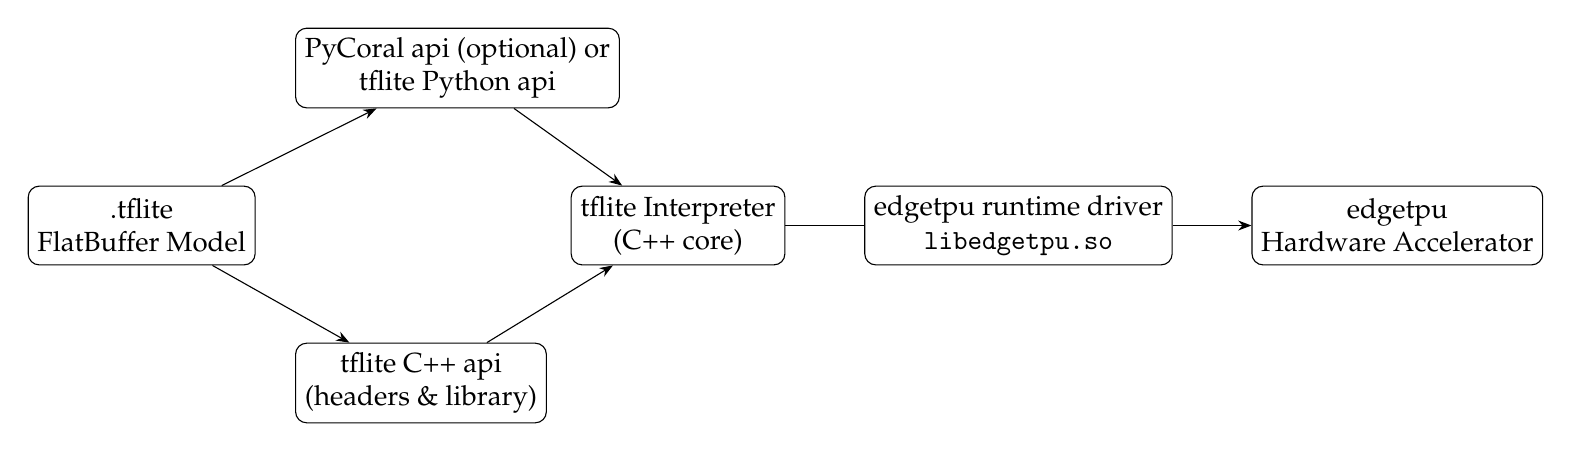
\begin{tikzpicture}[
  >=Stealth, ->,
  box/.style={rectangle,draw,rounded corners,
              minimum width=1cm,minimum height=1cm,
              align=center,font=\normalsize}
]

% Shared start
\node[box] (model) {.tflite\\FlatBuffer Model};

% API branches
\node[box, right=0.5cm of model, yshift=2cm] (pyapi) {PyCoral \gls{api} (optional) or\\\gls{tflite} Python \gls{api}};
\node[box, right=0.5cm of model, yshift=-2cm] (cppapi) {\gls{tflite} C++ \gls{api}\\(headers \& library)};

% Convergence
\node[box, right=4cm of model] (interp) {\gls{tflite} Interpreter\\(C++ core)};

% Runtime + hardware
\node[box, right=1cm of interp] (runtime) {\gls{edgetpu} runtime driver\\\texttt{libedgetpu.so}};
\node[box, right=1cm of runtime] (hw) {\gls{edgetpu}\\Hardware Accelerator};

% Connections
\draw (model) -- (pyapi);
\draw (model) -- (cppapi);
\draw (pyapi) -- (interp);
\draw (cppapi) -- (interp);
\draw (interp) -- (runtime) -- (hw);

\end{tikzpicture}%
}
\caption{Running the model on \gls{edgetpu} with Python and C++}
\label{fig:runflow}
\end{figure}

Since no prebuilt \gls{tflite} C++ \gls{api} libraries were available for the \gls{devboard}, it had to be built from source.
The process is described in detail in \secshortref{subsec:tecchallDeployment}
and marks the third and final technical implementation challenge in this work.

After successfully incorporating the \gls{tflite} C++ \gls{api} on the \gls{devboard},
it was used to implement the first C++ inference in \code{inference.cpp}.
Following this, a folder-reading utility was implemented in C++ to process multiple patches sequentially.
These patches are stored as \code{.bin} files with known shape and data type (\gls{float32}).
After inference, the program writes \code{.bin} outputs containing the predicted cloud masks in \gls{float32}.
Quantization parameters for the input and output are retrieved from the model at runtime and used to quantize the input tensor and dequantize the output tensor.
Later, the stitching process was also implemented in C++.
By running \code{stitch.cpp}, all \code{.bin} patches in the input folder are stitched into a single \code{.bin} scene without gaps.
This \code{.bin} scene can then be converted to a \code{.png} for visual inspection.
This conversion can optionally be performed on the \gls{devboard} using the Python script \code{convert.py}.

Note that the entire inference, stitching, and conversion pipeline could have been consolidated into a single C++ executable.
It was intentionally kept separate for two reasons:
(i) to allow greater flexibility and lower overhead for a future performance-critical satellite implementation, and
(ii) because the persistent error described in \secshortref{subsec:tecchallDeployment} prevents running any code immediately after the inference step.

As final steps concluding the inference implementation on the \gls{devboard}, the following improvements were made.
An SD card containing prepared \code{.bin} patches for each scene is mounted on the \gls{devboard},
allowing the entire dataset (several~GB) to be hosted, otherwise infeasible on the \gls{devboard}'s internal storage.
The stitching and conversion processes were unified under a single executable: after C++ \code{.bin} stitching, a Python function is invoked to perform the conversion.
During both inference and stitch-conversion processes, the user is prompted to select one of the 20 test scenes for inference and/or conversion.
Furthermore, the Python \code{.png} conversion was improved by avoiding loading the entire output array into the \gls{devboard}'s \gls{ram}.
Instead, chunked processing is used, enabling conversion of larger full resolution scenes.

\subsection*{Technical Challenges}
\label{subsec:tecchallDeployment}

The final significant implementation milestone in this work was building the \gls{tflite} C++ \gls{api} library for the \gls{devboard} from source.
As shown in \autoref{fig:runflow}, this library is crucial for implementing pure C++ inference.

Guidance for this task is only sparsely mentioned in the official documentation\footnote{\url{https://coral.ai/docs/edgetpu/tflite-cpp/\#build-your-project-with-libedgetpu}}.
Taking those notes into account, a compatible \gls{tflite} version for the \code{libedgetpu} runtime preinstalled on the \gls{devboard} had to be determined.
The installed \code{libedgetpu} was identified as v16.0. However, the releases page\footnote{\url{https://github.com/google-coral/libedgetpu/releases}}
does not use a consistent numeric versioning convention, so the modification date of the \code{libedgetpu.so.1} symlink was used to approximate the release.
On the \gls{devboard} used here this date was 09.07.2021,
which predates the official “Grouper” \code{libedgetpu} release\footnote{\url{https://github.com/google-coral/libedgetpu/tree/release-grouper}} (26.07.2021) by two weeks.
From that release's \code{workspace.bzl}, the exact \gls{tf} commit corresponding to \gls{tf}~2.5.0 (05.07.2021) was identified.

The first build attempt was performed on a Windows machine via cross-compilation for \code{aarch64} Linux.
Although compilation succeeded, the first inference test failed due to low-level incompatibilities with the \gls{devboard}'s atomic instructions.
It was therefore concluded that the library must be built either with Bazel using a full \gls{devboard} configuration or directly on the device.
The latter was chosen. An SD card was used to host the large \gls{tf} source tree (specific v2.5.0 commit) and to provide swap space,
to avoid running out of \gls{ram} during compilation. The build was performed using the then-latest portable \code{CMake}.

After successfully building the static library \code{libtensorflow-lite.a}, several additional steps were required.
The \code{edgetpu.h} header\footnote{\url{https://github.com/google-coral/libedgetpu/blob/master/tflite/public/edgetpu.h}} and a FlatBuffers library (v1.12.0) compatible with the build were obtained,
and all required \gls{tflite} static libraries were included.
The necessary include paths and libraries are recorded in the repository and can also be reviewed in the \code{MAKEFILE}.

Once compiler and linker issues were resolved and all requirements satisfied, successful model loading and tensor allocation using the C++ \gls{api}
marked the final technical milestone of this work.

\subsubsection*{Open Issue}

In the scope of this work, and with regard to the specific \gls{devboard} with its installed Mendel Linux OS and modules, an unusual behaviour after inference was observed.
From early development through the final C++ inference improvements, one of two errors persistently appeared only after the inference had completed:
\code{Segmentation fault} or \code{Bus error}.
The phenomenon was first encountered during the simple proof-of-concept Python inference, at program termination after results had been successfully saved.
Although such errors are typically disastrous, their occurrence at shutdown had no effect on obtaining the required inference outputs.
As they clearly originated in C++ backend code, debugging from Python was not feasible; nonetheless, pipeline development proceeded unaffected.

The move to a pure C++ inference was motivated in part by the desire to eliminate these errors.
However, even after the first successful C++ results, the errors continued to alternate upon exiting \code{main()} in \code{inference.cpp}.
During debugging, the source was narrowed down to the \code{libedgetpu} library --- presumably during its cleanup routine after inference.
Exact lines could not be traced, as the provided \code{libedgetpu} was built without debugging symbols.
Diagnosing this would require rebuilding the library with debug information, a process likely to entail dependency issues and other challenges typical of custom low-level builds.
This appears to be a worthwhile line of investigation but lies beyond the scope of this thesis.
It is presumed that the issue was fixed in later \code{libedgetpu} releases\footnote{\url{https://github.com/tensorflow/tensorflow/issues/62371}},
but without an official upgrade path on the device, a custom rebuild would have been inevitable.

Work was therefore continued, as the errors had no impact on performance or results.
Multiple \code{Interpreter} invocations can be executed to process folders of files. However, no code can be run after inference completes, because the program crashes at exit.
Consequently, the stitching and conversion stages were implemented as separate programs.

\section{Evaluation Pipeline}
\label{sec:evaluation}

With the implementation of the deployment pipeline on the \gls{devboard}, cloud prediction masks can be obtained.
Visual inspection by a human observer is used to qualitatively confirm successful implementation and attainment of the thesis objective.
Furthermore, a quantitative performance metric was implemented in \code{inference.cpp} on the \gls{devboard} to determine the inference time per processed patch;
by summing these times, the model's per-scene inference time is obtained.

The flexibility of the training and deployment pipelines allows convenient, modular improvement and feature expansion.
They can be tailored to the needs and requirements of model development intended for immediate satellite deployment.
For this, additional quantitative evaluation of model performance is necessary. The results are ultimately used in \secshortref{chapter:evaluation},
where the performance of several \gls{edgetpu} optimized models is assessed.

The evaluation pipeline is implemented as an additional stage following the training pipeline and is run on the training machine, not on the \gls{devboard}.
The evaluation pipeline consists of two parts: inference and evaluation.

\subsection*{Inference}

The necessary functions to perform inference and save results are implemented in the files \code{inference.py} and \code{inferenceQ.py}.
\code{inferenceQ.py} uses the \gls{tflite} \code{Interpreter} with the fully \gls{int8} quantized \code{.tflite} model,
whereas \code{inference.py} relies on \gls{tf} utilities and loads the \code{.h5} saved-model format.
It was observed that running the quantized model on a \gls{cpu} results in significantly slower inference than the \gls{float32} \code{.h5} model, which slows down the evaluation.
Moreover, executing the quantized model on a general-purpose \gls{cpu} Intel Core i5-13400F yielded inference times even slower than deployment on the dedicated \gls{edgetpu}.
This inherently emphasizes the sophistication of the \gls{tpu} in performing these operations, compared to a general-purpose \gls{cpu} that is otherwise more powerful for general tasks.
Consequently, quantized inference was omitted during evaluation, and \code{inference.py} is used for the remainder.

First, the \code{buildDS} function is used to construct the testing dataset.
As mentioned in \secshortref{subsec:testing}, prebuilt \code{.csv} files are used to assemble either a single-scene dataset (specified by ID or chosen at random) or the full test set.
In later versions of \code{inference.py}, full-dataset inference is handled internally on a scene-wise basis, reducing \gls{ram} usage and preventing crashes.
Accordingly, \code{fullTestDS.csv} is no longer used.
Next, the path to the desired \code{run} folder (containing the \code{.h5} and \code{.tflite} files) is specified.
In \code{inference.py} the \code{.h5} model is loaded, providing any required custom \gls{tf} objects (e.g., \code{softJaccardLoss}, \code{diceCoefficient}).

If model predictions are produced at reduced resolution (e.g., \(\,192\times192\,\) patches),
they are upsampled to the full \(\,384\times384\,\) resolution to match full-scene \glspl{gt} during evaluation.
Upsampling is performed with \code{bilinear} interpolation (see also \secshortref{sec:data}),
which is appropriate for continuous probability maps.

Finally, the inference results are saved per scene as \code{.npy} files for use in the evaluation process.
Optionally, masks can also be saved as \code{.png} files for visual inspection.

\subsection*{Evaluation}

After obtaining inference results for the complete test set (20 scenes), they are quantified using the evaluation metrics defined in \secshortref{subsec:evalmetrics},
as implemented in \code{evaluate.py} file.
By specifying the \code{run} folder, that contains the \code{evaluation/inference} subfolder,
the algorithm locates and processes each scene's \code{.npy} file produced by the inference step.

As mentioned in \secshortref{subsec:dataset}, the test input scenes were cropped and padded to fit the \(\,384\times384\,\) patch format.
This introduces zero padding at the scene borders. To restore the original scene size of the \gls{gt} masks, the border padding must be removed.
This is performed by center-cropping the prediction masks via the helper function \code{unpadToMatch},
following the procedure used in the original dataset papers \cite{CloudNet2019, CloudDet2018} (cf. their \code{unzeropad} routine used
for evaluation\footnote{\url{https://github.com/SorourMo/38-Cloud-A-Cloud-Segmentation-Dataset/blob/master/evaluation/evaluation.m}}).

Next, the evaluation pipeline offers two ways to choose the threshold (see \secshortref{subsec:evalmetrics}) for binarizing the predicted masks:
(i) apply the best threshold estimated on the validation set, or
(ii) determine the best threshold per test scene using its \gls{gt} mask.
The effects of these choices are discussed in the next \secshortref{chapter:evaluation}.
This functionality is controlled via the optional \code{fixedThreshold} argument to \code{evaluateAll} function.

As a final step, the prediction masks are binarized and metrics are computed using \code{computeMetrics} function.
Results are saved to \code{metricsValThr.csv} or \code{metricsTestThr.csv}, depending on the thresholding variant.
Optionally, per-scene \code{.npy} results can be saved alongside \code{.png} masks for visual inspection.

This process concludes the \emph{Implementation} chapter and finalizes the software development conducted within the scope of this work.

}
{

\setlength{\parindent}{0pt}
\setlength{\parskip}{1em}

\chapter{Evaluation}
\label{chapter:evaluation}

An implemented flexible pipeline gives the opportunity to conveniently train, convert and deploy various different model configurations for \gls{devboard}.
It enables fast switching between model's architecture, training and deployment configurations, for instance:
utilizing different number of input channels, changing the spatial resolution of input tensor, utilizing different training, validation, and testing subsets.
Tailoring these configurations to user needs requires only minor changes to pipeline code.

During the development process, numerous model architectures were designed and trained. Most of them served as prototypes for the debugging process.
For instance, the model \code{simple} yielded the first inference results, that are presented in \secshortref{sec:deployment}.
After successful implementation phase, five models were selected for the evaluation process. These models were trained for an appropriate number of epochs,
their inference time performance was checked on \gls{devboard} and evaluation metrics gathered utilizing evaluation pipeline. 
One of these model was the first to yield qualitatively high results.
It hosts a simplified and adjusted for edge inference \code{Cloud-Net} architecture\cite{CloudNet2019}.
The first model's architecture will be called \code{earlyCloudEdgeQ} in the scope of this work.
The remaining four models are all of the exact same architecture, which is an improved version of \code{earlyCloudEdgeQ}.
Architecture of these models is therefore called \code{improvedCloudEdgeQ}.
But these models are utilizing different number of input channels (\gls{rgb} with \gls{nir} or only \gls{rgb}),
and they furthermore are using different input patch size (either \ensuremath{192\times192} or \ensuremath{384\times384}).
It has to be mentioned, that all five of these models follow classical \code{uNet} structure,
outlined in \secshortref{subsec:stateoftheart}. They contain encoder, bottleneck and decoder,
as well as the skip-connections between corresponding encoder and decoder blocks.


Below the detailed description of both architectures is presented:
\begin{itemize}
    \item \textbf{earlyCloudEdgeQ}: The model hosts three encoder blocks, a bottleneck block, and three decoder blocks.
    Each encoder block consists of two \code{Conv2D} layers and one \code{MaxPooling2D} layer,
    connected sequentionally one after another. Bottleneck consists of two sequentionally connected \code{Conv2D} layers.
    Each decoder block is represented by \code{Conv2DTranspose} layer, \code{Concatenate} layer, and two \code{Conv2D} layers,
    connected sequentionally. An output layer is represented by a \code{Conv2D} layer.
    Base number of filter is specified as 32 and is doubled/halved in each encoder/decoder block respectively, resulting in 256 filters in the bottleneck.
    \gls{bn} is applied accordingly after each \code{Conv2D} layer, but before its activation function. \gls{bn} is not applied in output layer.
    All suitable \glspl{tfop} are \gls{qat} annotaded. \gls{bce} is used as loss function and \code{adam} \cite{adam} is used as optimizer.
    \item \textbf{improvedCloudEdgeQ}: This model mimics the previous architecture with the following improvements.
    Between input and first encoder block a \code{Conv2D} layer with 16 filters is added to improve feature representation at the input stage,
    enabling the encoder to capture more consistent low-level patterns before deeper processing.
    Furthermore the model hosts now four encoder blocks, a bottleneck block, and four decoder blocks. The bottleneck design was adapted from \code{Cloud-Net},
    where a residual connection with a $1\times1$ projection ensures feature dimension alignment and efficient gradient flow. Additionally,
    the integration of dropout regularization reduces overfitting, resulting in a more robust and generalizable feature representation at the network's deepest layer.
    These ideas are copied from \code{Cloud-Net} architecture.
    To meet the limited \gls{edgetpu} \gls{sram} capacity, the decoder blocks were simplified by removing one \code{Conv2D} layer from each block,
    except for the final decoder block before the output layer, which retains two \code{Conv2D} layers to preserve finer spatial resolution.
    Additionally, using \gls{bce} combined with \ensuremath{0.5 \cdot DiceLoss} as the loss function balances pixel-wise accuracy with overlap-based region matching,
    leading to better segmentation performance than plain \gls{bce} \cite{bcedice1, bcedice2}.

\end{itemize}

\code{improvedCloudEdgeQ} architecture can be summarized as an adjusted \code{Cloud-Net} model to meet the contraints of embedded \gls{edgetpu} development.
Necessary simplifications were made. Both \code{earlyCloudEdgeQ} and \code{improvedCloudEdgeQ} architectures can be investigated more detailed in the
\code{model.py} file,
as well as compared with \code{Cloud-Net} model
architecture\footnote{\url{https://github.com/SorourMo/Cloud-Net-A-semantic-segmentation-CNN-for-cloud-detection/blob/master/Cloud-Net/cloud_net_model.py}}.

Following table further specifies the differencec between the models, providing information about number of input channels (CH),
size of an input patch (In size), number of training epochs (Epochs), estimated count of arithmetic operations in billions (Ops (B)),
On-chip/Off-chip memory used for caching model parameters (On-chip (MB)/Off-chip (KB)),
inference time needed by \gls{devboard} to process one batch in milliseconds (Inf. Time (ms)).

\begin{table}[h!]
\centering
\caption{Comparison of model properties and deployment metrics}
\label{tab:model_comparison}
\renewcommand{\arraystretch}{1.3}
\resizebox{\textwidth}{!}{%
\begin{tabular}{|l|c|c|c|c|c|c|c|}
\hline
\textbf{Model} & \textbf{CH} & \textbf{In size} & \textbf{Epochs} & \textbf{Ops (B)} & \textbf{On-chip (MB)} & \textbf{Off-chip (KB)} & \textbf{Inf. Time (ms)} \\ \hline
early      & 4 & 192 & 100  & 10.4 & 1.9 & 46  & 15.2 \\ \hline
improved~1 & 3 & 192 & 54   & 11.6 & 5.7 & 342 & 20.5 \\ \hline
improved~2 & 3 & 384 & 46   & 46.3 & 6.0 & 349 & 12.7 \\ \hline
improved~3 & 4 & 192 & 51   & 11.6 & 5.7 & 342 & 10.3 \\ \hline
improved~4 & 4 & 384 & 45   & 46.4 & 6.0 & 349 & 25.8 \\ \hline
\end{tabular}%
}
\end{table}

\todo{inference time coral and add learnable params!}

Models were evaluated on a test set, containing 20 scenes. The evaluation metrics, outlined in \secshortref{subsec:evalmetrics}
were calculated per scene and then averaged:
IoU, Dice Coefficient, Precision, Recall, Accuracy. Averaging does not skew the results, because all scene are of approximately the same size.
Furthermore, for each model except \code{early} the best binarization threshold was calculated immediately after the training precess,
utilizing the bestF1 score, obtained on a validation set.
This improves model to be inference-ready with its own calibrated best threshold for immediate binarization of predicted masks.
For \code{early} model no threshold was calculated, since to the point of its training, the feature was not yet implemented.
Features for the reproducibility of shuffling the datasets were not implemented at the time too,
leaving no chance to perform \code{PRC} evaluation on the same validation set to make up for the best validation threshold.
In addition to determining the optimal threshold from the validation set,
a per-scene threshold was computed individually for each of the 20 test scenes and subsequently averaged.
This procedure is even more optimistic than selecting a single global test threshold,
since it implicitly adapts to each test scene and therefore overestimates true generalization performance.
Nonetheless, presenting these results is useful, as it illustrates the upper bound of performance
achievable under ideal threshold tuning and underscores the strong influence of threshold choice on segmentation quality.
The final evaluation results are represented on three column chart below,
whereas second and third charts are derived from the first one, splitting between validation set threshold and test set threshold
for better visual comparison possibility.
\code{improvedCloudEdgeQ} models are represented only by their parameters configuration, such as number of input channels and input patch' size,
\code{earlyCloudEdgeQ} is highlighted additionally as \code{early} model. 

\begin{figure}[H]
  \centering
  \includegraphics[width=\textwidth]{files/evalRes.pdf}
  \caption{The basic workflow to create a model for the Edge TPU}
  \label{fig:evalres}
\end{figure}

\begin{figure}[H]
  \centering
  \begin{subfigure}[t]{\textwidth}
    \centering
    \includegraphics[width=\textwidth,height=0.45\textheight,keepaspectratio]{files/valSetThr.pdf}
    \caption{Links}
  \end{subfigure}
  \vspace{0.8em}
  \begin{subfigure}[t]{\textwidth}
    \centering
    \includegraphics[width=\textwidth,height=0.45\textheight,keepaspectratio]{files/testSetThr.pdf}
    \caption{Rechts}
  \end{subfigure}
  \caption{Zwei Diagramme übereinander (als PDF).}
\end{figure}

By analizing these results, following key insights can be made:
\begin{itemize}
    \item A general upward performance trend can clearly be seen with increasing input patch resolution and with addition of \gls{nir} channel.
    This is expected, as the model benifits from additional input information sources.
    \item \code{improvedCloudEdgeQ} architecture performs generally better than \code{earlyCloudEdgeQ} given the architecture improvements.
    \item At input size \ensuremath{192\times192}, adding the \gls{nir} channel did not improve recall and in fact led to a slight reduction,
    when analizing the validation threshold. This effect likely arises because the additional spectral information increases input dimensionality without
    providing sufficient spatial context at the lower resolution. As a result, the model becomes more conservative at cloud boundaries and thin structures,
    which reduces false positives but slightly increases the number of missed cloud pixels, leading to lower recall.
    \item The accuracy metric is constanltly at a very high level, but it has better not to be qualified as a reliable metric in the
    cloud segmentation case, as explained in \secshortref{subsec:evalmetrics}. <TODO EXPLAIN THERE>
\end{itemize}

Based on the evaluation metrics and taking the inference time on \gls{devboard} into consideration the \code{improvedCloudEdgeQ} model,
with \gls{rgb} and \code{nir} input channels as well as \ensuremath{192\times192} spatial resolution, is proposed as the best suitable model
out of all trained and evaluated models in the scope of this work. This model represents the golden middle between edge device inference speed
and performance metrics.
However, if the input data lacks \code{nir} channel, providing only \code{rgb} imagery, the best model is chosen to be
\code{improvedCloudEdgeQ} of \ensuremath{384\times384}, trading significantly increased inference time for the more than acceptable performance.

}
{

\setlength{\parindent}{0pt}
\setlength{\parskip}{1em}

\chapter{Conclusions \& Outlook}

}

% Optional start of thesis content
\clearpage
\setlength{\parindent}{0pt}
\setlength{\parskip}{1em}

\printbibliography
\end{document}